% This is samplepaper.tex, a sample chapter demonstrating the
% LLNCS macro package for Springer Computer Science proceedings;
% Version 2.20 of 2017/10/04
%

\documentclass[runningheads]{llncs}
\raggedbottom
%
\usepackage[utf8]{inputenc}
\usepackage[utf8]{vietnam}
\usepackage{graphicx}
\usepackage{epstopdf}
\usepackage{float}
\usepackage{array}
\usepackage{multirow}
\usepackage{ulem}
\usepackage[hyphens]{url}
\usepackage{todonotes}
\usepackage{listings}
\usepackage{xcolor}
\usepackage{fancyvrb}
\usepackage{verbatimbox}

\lstset{
    literate={~} {$\sim$}{1}
}

\definecolor{cverbbg}{gray}{0.93}

\newenvironment{cverbatim}
 {\SaveVerbatim{cverb}}
 {\endSaveVerbatim
  \flushleft\fboxrule=0pt\fboxsep=.5em
  \colorbox{cverbbg}{\BUseVerbatim{cverb}}%
  \endflushleft
}

\newenvironment{lcverbatim}
 {\SaveVerbatim{cverb}}
 {\endSaveVerbatim
  \flushleft\fboxrule=0pt\fboxsep=.5em
  \colorbox{cverbbg}{%
    \makebox[\dimexpr\linewidth-2\fboxsep][l]{\BUseVerbatim{cverb}}%
  }
  \endflushleft
}

\newenvironment{fullgrayverb}
{\verbbox}
{\endverbbox\par\colorbox{lightgray}{\parbox{\textwidth}{\theverbbox}}\par}


% Used for displaying a sample figure. If possible, figure files should
% be included in EPS format.
%
% If you use the hyperref package, please uncomment the following line
% to display URLs in blue roman font according to Springer's eBook style:
% \renewcommand\UrlFont{\color{blue}\rmfamily}

\begin{document}
%
\title{Phân tích ảnh hưởng của các chỉ số sức khỏe đến tiến triển bệnh đái tháo đường \thanks{Hướng dẫn bởi TS. Đỗ Trọng Hợp}}
%
%\titlerunning{Abbreviated paper title}
% If the paper title is too long for the running head, you can set
% an abbreviated paper title here
%
\author{Thái Minh Triết\inst{1} \and
Chu Hà Thảo Ngân\inst{2} \and
Võ Tuấn Anh\inst{3} \and
Đỗ Trọng Hợp\inst{4}
}
%
\authorrunning{Thái Minh Triết, Chu Hà Thảo Ngân , Võ Tuấn Anh}
% First names are abbreviated in the running head.
% If there are more than two authors, 'et al.' is used.
%
\institute{Trường Đại học Công nghệ thông tin, Đại học quốc gia Thành phố Hồ Chí Minh \and
Khoa Khoa học và Kỹ thuật Thông tin\\
\email{\{\inst{1}19522397,\inst{2}19521882,\inst{3}19521226\}@gm.uit.edu.vn\\
{\inst{4}hopdt}@uit.edu.vn}\\Nhóm 9}

%
\titlerunning{Phân tích ảnh hưởng của các chỉ số sức khỏe đến bệnh tiểu đường}
\maketitle              % typeset the header of the contribution
%
\begin{abstract}
Bệnh đái tháo đường theo giới y khoa là một trong những mối đe doạ sức khoẻ toàn cầu đối với cộng đồng có tỉ lệ người mắc ngày càng tăng đều theo từng năm với nhiều nguyên nhân ảnh hưởng, trong đó nguyên nhân chính là rối loạn chức năng chuyển hóa insulin. Nhằm tìm hiểu được các yếu tố bên trong cơ thể có tác động như thế nào đến sự rối loạn này, nhóm chúng tôi đã tìm hiểu các chỉ số y tế mang tính thống kê có liên quan bằng bộ dữ liệu có sẵn và tiến hành phân tích, xử lí và đánh giá để có được những kết quả phù hợp cho mục đích của bài nghiên cứu. Trong quá trình phân tích có sử dụng phương pháp thống kê phân tích hồi quy để tìm ra sự ảnh hưởng và tương tác lẫn nhau của các yếu tố này. Sau khi thực hiện xây dựng các mô hình hồi quy phù hợp và đánh giá chúng, kết quả thu được trên độ đo đánh giá Adjusted R-Squared là 0.5795  cho mô hình phân tích tốt nhất là mô hình Multiple Linear Regression trên tập dữ liệu kiểm thử chưa qua tiền xử lý. 

\keywords{Bệnh đái tháo đường \and Bệnh tiểu đường \and  Phân tích hồi quy}
\end{abstract}
%
%
%
\section{Giới thiệu chung}

Đái tháo đường được xem là một căn bệnh phổ biến trong cộng đồng, đặc biệt là Mỹ với xu hướng gia tăng ngày càng cao với con số ước tính lên đến 79 triệu người trưởng thành mắc bệnh và trong đó 50\% người mắc đái tháo đường không biết mình có bệnh vì chưa có triệu chứng rõ ràng. 

Đái tháo đường là một căn bệnh liên quan đến sự rối loạn chuyển hóa trong hormone tuyến tuỵ dẫn đến thiếu hụt lượng insuline trong máu. Các tiêu chuẩn để xác định, chẩn đoán bệnh đái tháo đường hiện nay được Hiệp hội Đái tháo đường Mỹ công bố cần dựa vào nhiều chỉ số và quá trình phức tạp. Ví dụ khi kiểm tra chỉ số HbA1c của bệnh nhân cần được thực hiện ở phòng thí nghiệm được chuẩn hóa cao. Tuy nhiên, cũng nhờ đó mà việc chẩn đoán đái tháo đường hay tiền đái tháo đường sẽ phần lớn phụ thuộc vào các chỉ số này từ cơ thể. 
Chính vì đó, ta cần phải có được một bộ dữ liệu với các chỉ số y tế liên quan để có thể đánh giá phần nào tình trạng hiện tại của bệnh, giúp tăng hiệu quả cũng như giảm đi chi phí cho quá trình chuẩn đoán. 

Trong bài nghiên cứu này, chúng tôi phân tích ảnh hưởng giữa các yếu tố là chỉ số y tế liên quan lên tiến triển bệnh và tương tác giữa các yếu tố này được thu thập từ các bệnh nhân đái tháo trong bộ dữ liệu sẵn. Sau đó chúng tôi xây dựng các mô hình hồi quy và đánh giá kết quả dự đoán của các mô hình. Từ đó không chỉ hỗ trợ tích cực cho việc chẩn đoán mà còn phân tích được tiến triển của bệnh qua các chỉ số trên.

Cấu trúc bài báo cáo được trình bày như sau: Ở mục 2, chúng tôi trình bày thông tin chi tiết của bộ dữ liệu được sử dụng trong bài nghiên cứu. Ở mục 3, chúng tôi tiếp cận bộ dữ liệu và thực hiện tiền xử lý dữ liệu. Sau khi bộ dữ liệu đã được xử lý, chúng tôi sẽ phân tích ảnh hưởng và tương tác yếu tố trong bộ dữ liệu và chúng sẽ được đưa vào phân tích bằng các mô hình hồi quy khác nhau, quá trình này sẽ được trình bày ở mục 4. Mục 5 sẽ trình bày kết quả đánh giá các mô hình, từ đó có được mô hình tốt nhất trên bộ dữ liệu. Và cuối cùng ở mục 6 là kết luận và hướng phát triển.

\section{Tổng quan bộ dữ liệu}

\subsection{Giới thiệu chung về bộ dữ liệu}
Bộ dữ liệu được xây dựng bao gồm  thuộc tính cơ bản của 442 bệnh nhân bệnh tiểu đường và kết quả là một giá trị đáng giá quá trình tiến triển của bệnh nhân sau 1 năm ghi nhận. Dưới đây là ví dụ các điểm dữ liệu được trích ra từ bộ dữ liệu và codebook của bộ dữ liệu.
\begin{table}
	\setlength{\tabcolsep}{0.5em}
	\renewcommand{\arraystretch}{1.4}
	\begin{center}
		\caption{Ví dụ về các điểm dữ liệu}\label{tab1}
		\begin{tabular}{|p{0.75cm}|p{0.75cm}|p{0.75cm}|p{0.75cm}|p{0.75cm}|p{0.75cm}|p{0.75cm}|p{0.75cm}|p{1cm}|p{0.75cm}|p{0.75cm}|}
			\hline
			\textbf{AGE}&\textbf{SEX}&\textbf{BMI}&\textbf{BF}&\textbf{S1}&\textbf{S2}&\textbf{S3}&\textbf{S4}&\textbf{S5}&\textbf{S6}&\textbf{Y}\\
			\hline
			59&2&32.1&101&157&93.2&38&4&4.8598&87&151\\
			\hline
			48&1&21.6&87&183&103.2&70&3&3.8918&69&75\\
			\hline
			72&2&30.5&93&156&93.6&41&4&4.6728&85&141\\
			\hline
			24&1&25.3&84&198&131.4&40&5&4.8903&89&206\\
			\hline
			50&	1	&23&	101&	192&	125.4&	52&	4&	4.2905&	80&	135\\
			\hline
		\end{tabular}
	\end{center}
\end{table}

\begin{table}[H]
	\setlength{\tabcolsep}{0.5em}
	\renewcommand{\arraystretch}{1.4}
	\begin{center}
		\caption{Codebook của bộ dữ liệu}\label{tab2}
			\begin{tabular}{ | p{2.5cm} | p{9.45cm} |} 
			\hline
			\textbf{Thông tin} & \textbf{Nội dung}\\ 
			\hline
			Tên bộ dữ liệu &Diabetes dataset\\
			\hline
			Nguồn thu nhập & \url{https://www4.stat.ncsu.edu/~boos/var.select/diabetes.html}\\
			\hline
			Số điểm dữ liệu & 442\\
			\hline
			Số thuộc tính & 11\\
			\hline
			\multirow{1}{2.25cm}
			{Thông tin thuộc tính} & \textbf{AGE:} độ tuổi của bệnh nhân\\
								&\textbf{SEX:} giới tính của bệnh nhân \\
								& -  Giá trị 1 tương ứng với giới tính là Nam\\
								& -  Giá trị 2 tương ứng với giới tính là Nữ\\
								&\textbf{BMI:} Body Mass Index (chỉ số khối cơ thể)\\
								&\textbf{BP:}  average blood pressure (giá trị huyết áp trung bình)\\
								&\textbf{S1:} tổng lượng cholesterol trong huyết thanh (tc - total serum cholesterol)\\
								&\textbf{S2:} giá trị lipoprotein tỷ trọng thấp (ldl - low-density lipoproteins) \\
								&\textbf{S3:} giá trị lipoprotein tỷ trọng cao (hdl - high-density lipoproteins)\\
								&\textbf{S4:} tỉ lệ giữa  cholesterol toàn phần so với lượng HDL (tch - total cholesterol / HDL) \\
								&\textbf{S5:} mức triglycerides có trong huyết thanh có thể ghi nhận (ltg - possibly log of serum triglycerides level)\\
								&\textbf{S6:}  chỉ số mức đường huyết (glu - blood sugar level)\\
								&\textbf{Y:} giá trị định lượng về tiến triển bệnh của bệnh nhân sau 1 năm kể từ thời điểm ghi nhận\\
								\hline
			Tác giả & Bradley Efron, Trevor Hastie, Iain Johnstone và Robert Tibshirani, Đại học Stanford, Hoa Kỳ\\
			\hline
			\end{tabular}
		\end{center}
\end{table}

\subsection{Trực quan bộ dữ liệu}

Trước khi tiến hành phân tích các ảnh hưởng, việc trực quan hóa dữ liệu sẽ giúp chúng ta hiểu rõ phân bố của các điểm dữ liệu và mối quan hệ giữa các thuộc tính, hoặc có thể từ đó xem xét một thuộc tính có ý nghĩa thống kê hay không. Trực quan hóa giúp mô tả các dữ liệu thô thành hình ảnh dễ quan sát, dễ hiểu để truyền đạt rõ ràng những hiểu biết đầy đủ (insights) từ dữ liệu đến người xem, người đọc. Nếu không có sự trình bày trực quan này, người xem có thể khó nắm bắt được ý nghĩa thực sự của những phát hiện.

\pagebreak

\vspace{0.5cm}
\textbf{Thống kê mô tả các thuộc tính của bộ dữ liệu}
\begin{figure}[htb]
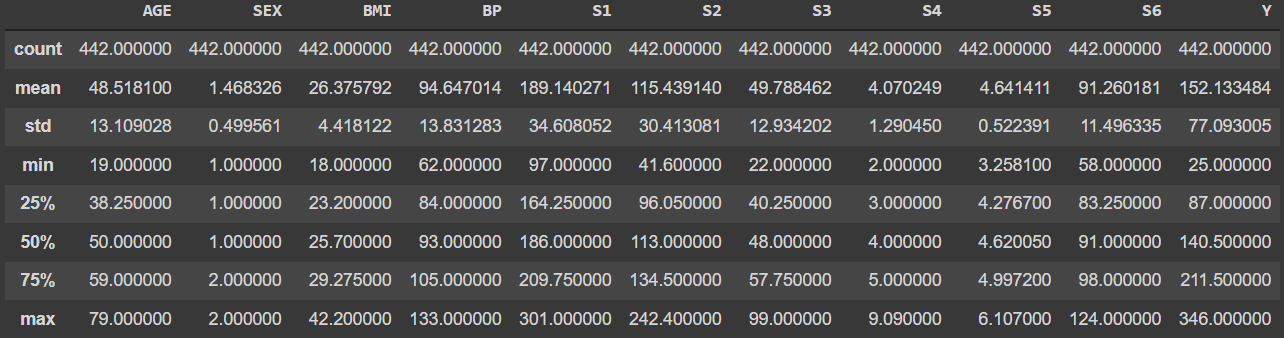
\includegraphics[width=1\textwidth]{describe}
\caption{Thống kê mô tả bộ dữ liệu} \label{fig1}
\end{figure}

\textbf{Biểu đồ phân tán của các thuộc tính so với thuộc tính Y}

\begin{figure}[H]
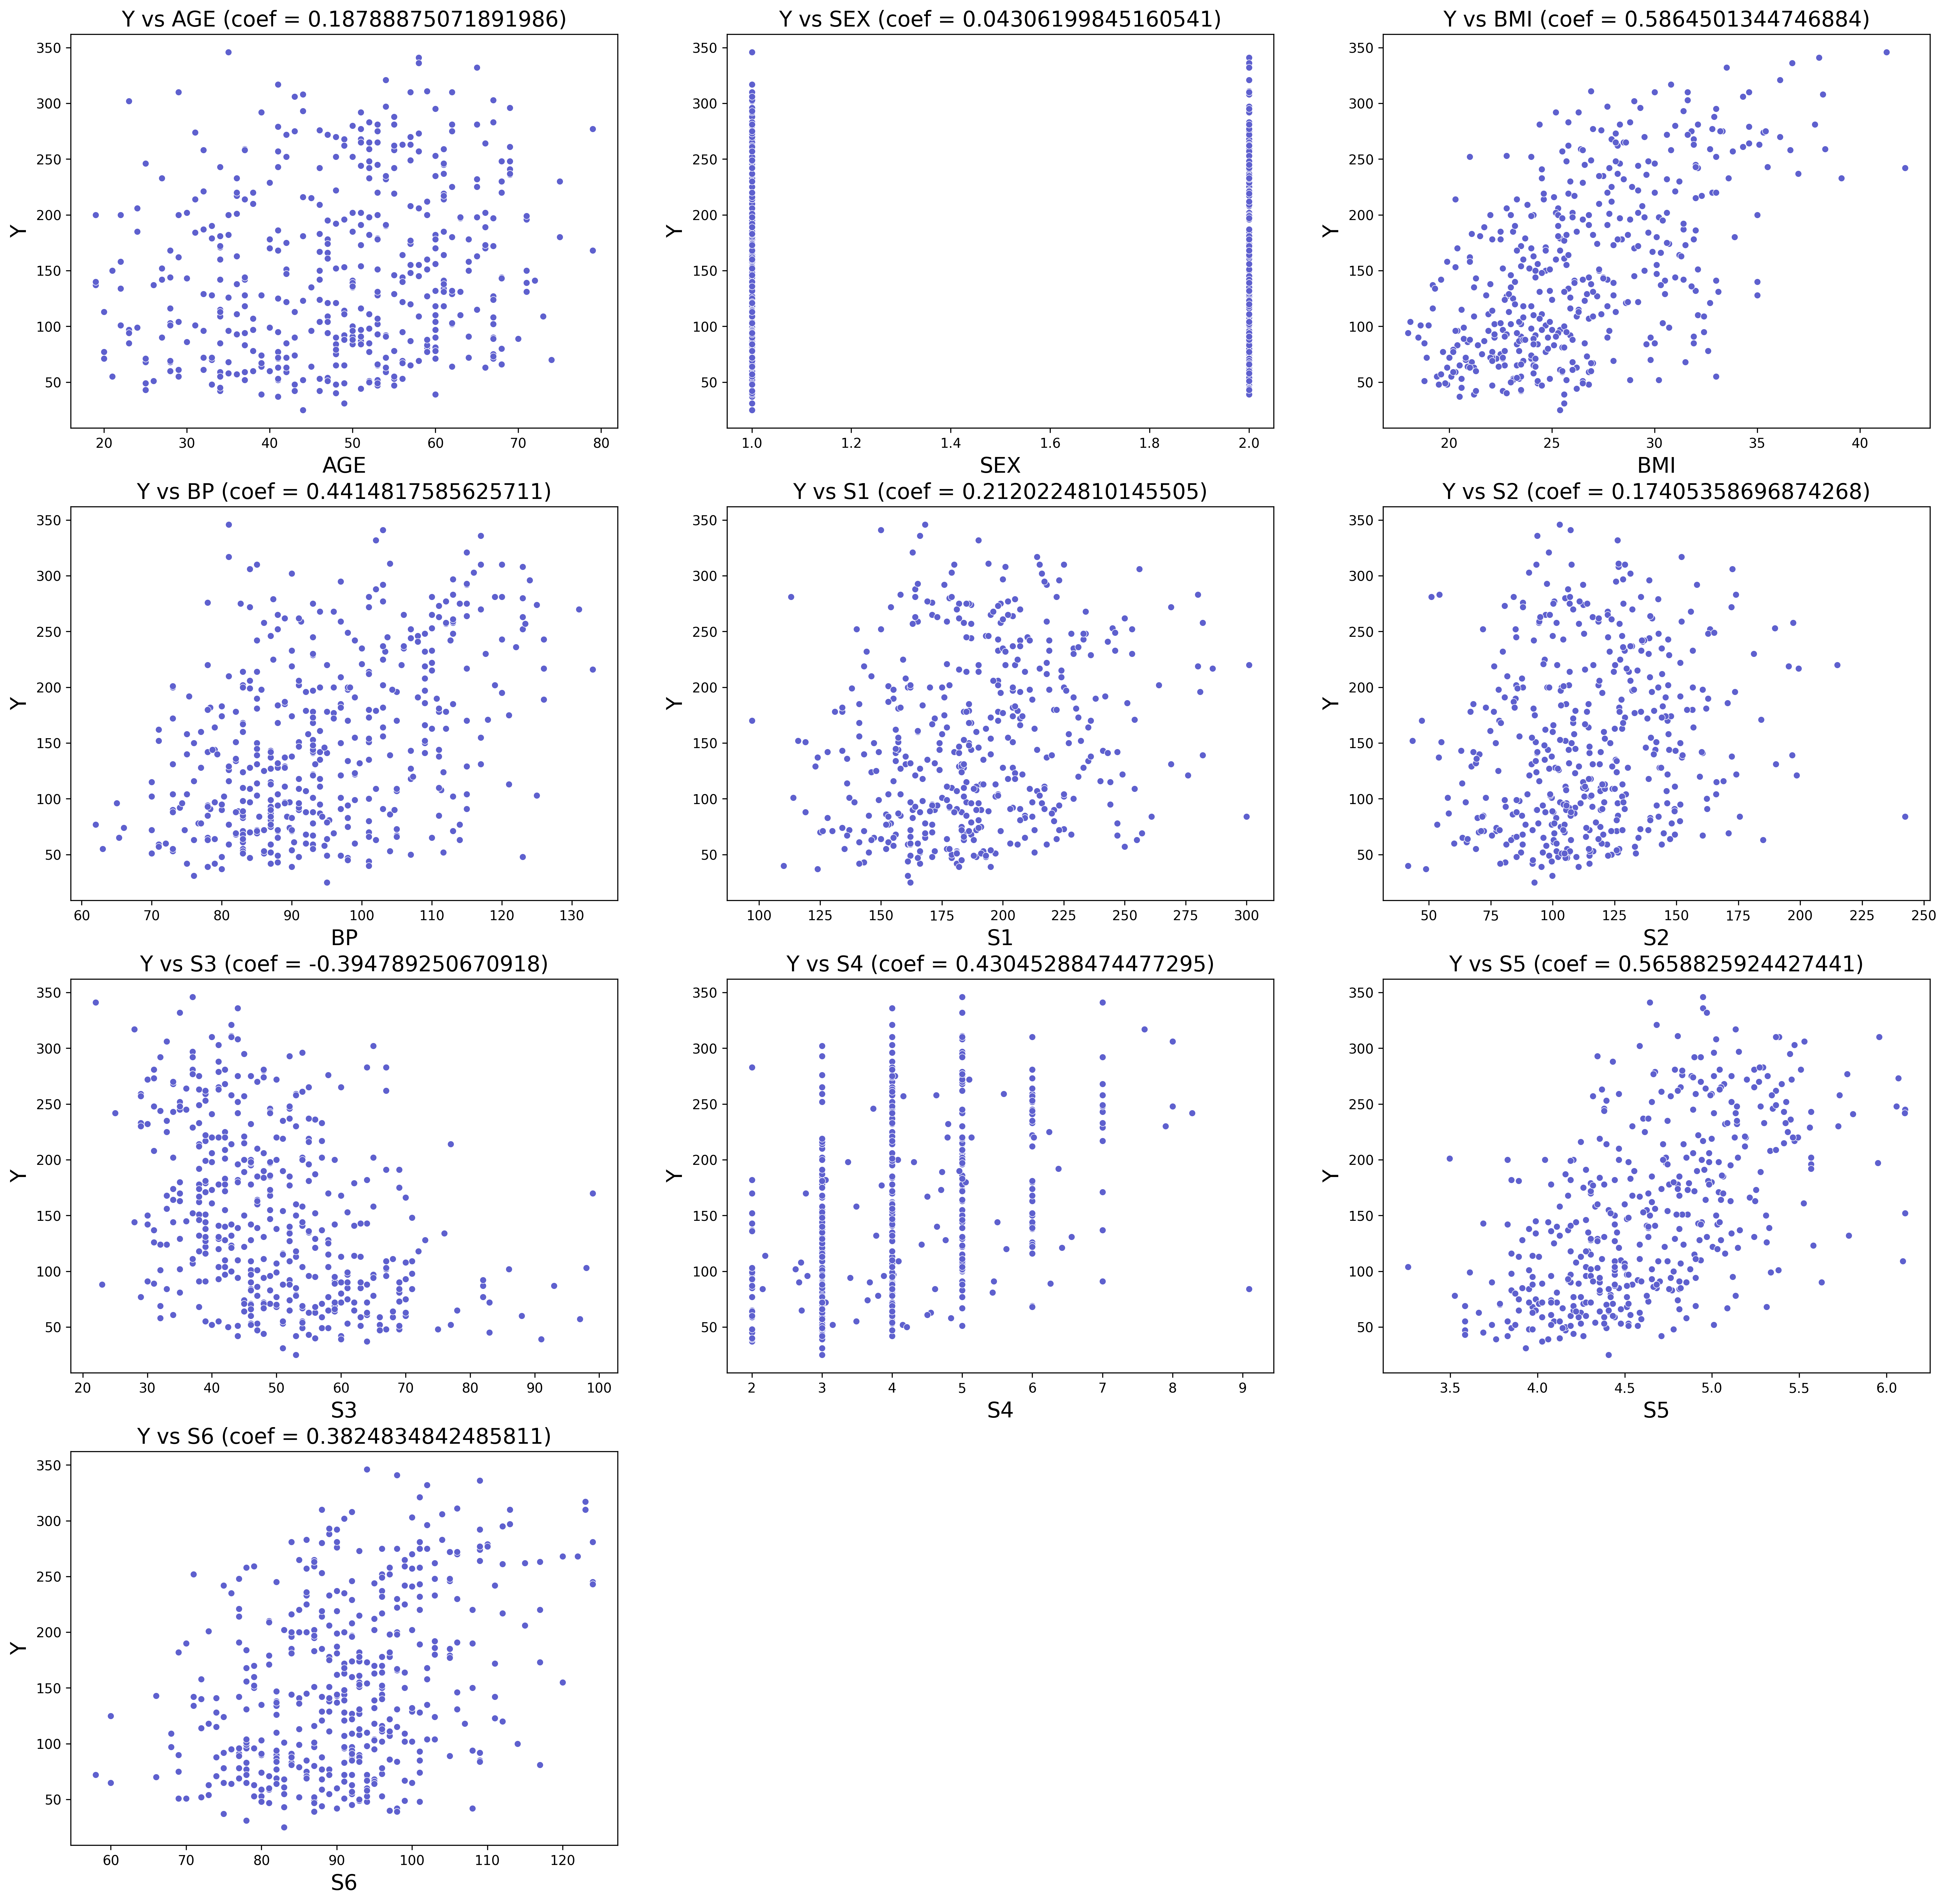
\includegraphics[width=0.955\textwidth]{Scatter_Y}
\caption{Biểu đồ phân tán của các thuộc tính so với thuộc tính Y} \label{fig2}
\end{figure}


Thông qua biểu đồ phân tán, chúng tôi nhận thấy ở các thuộc tính BMI và S5 phân bố điểm dữ liệu có xu hướng hội tụ về dạng đường thẳng. Các thuộc tính còn lại hầu như phân bố hỗn loạn và ít có quan hệ tuyến tính với thuộc tính Y.

Bên cạnh đó, biểu đồ phân tán cũng cho thấy được các điểm dữ liệu ngoại lệ ở thuộc tính S2 và S4, có thể ảnh hưởng đến hiệu suất của các mô hình hồi quy.

\vspace{0.5cm}
\textbf{Biểu đồ phân tán giữa các thuộc tính định lượng}

\begin{figure}[H]
\centering
\includegraphics[width=\textwidth]{Scatter_factors}
\caption{Biểu đồ phân tán giữa các thuộc tính định lượng} \label{fig2}
\end{figure}

Qua biểu đồ có thể thấy thuộc tính S1 có quan hệ tuyến tính rõ rệt với S2. Một số thuộc tính khác có quan hệ tuyến tính nhưng không nhiều như S2 và S4, S3 và S4, S6 và S5. Các biểu đồ còn lại đa số các điểm dữ liệu phân bố hỗn loạn không theo một quy luật cụ thể.

Ngoài ra, tương tác giữa các thuộc tính có những ảnh hưởng khác nhau giữa đến tiến triển bệnh. Ví dụ như ở biểu đồ của S5 so với BMI cho thấy những bệnh nhân có chỉ số BMi và S5 thấp thì tiến triển bệnh chậm, khi hai chỉ số này cùng tăng thì bệnh có khả năng thể tiến triển nhanh hơn. Mặt khác, ở biểu đồ của S3 so vớ BP, S3 cao nhưng BP thấp thì bệnh tiến triển nhẹ, S3 thấp nhưng BP cao cho thấy bệnh tiến triển nhanh.

\vspace{0.5cm}
\textbf{Biểu đồ hệ số tương quan}
\begin{figure}[H]
\centering
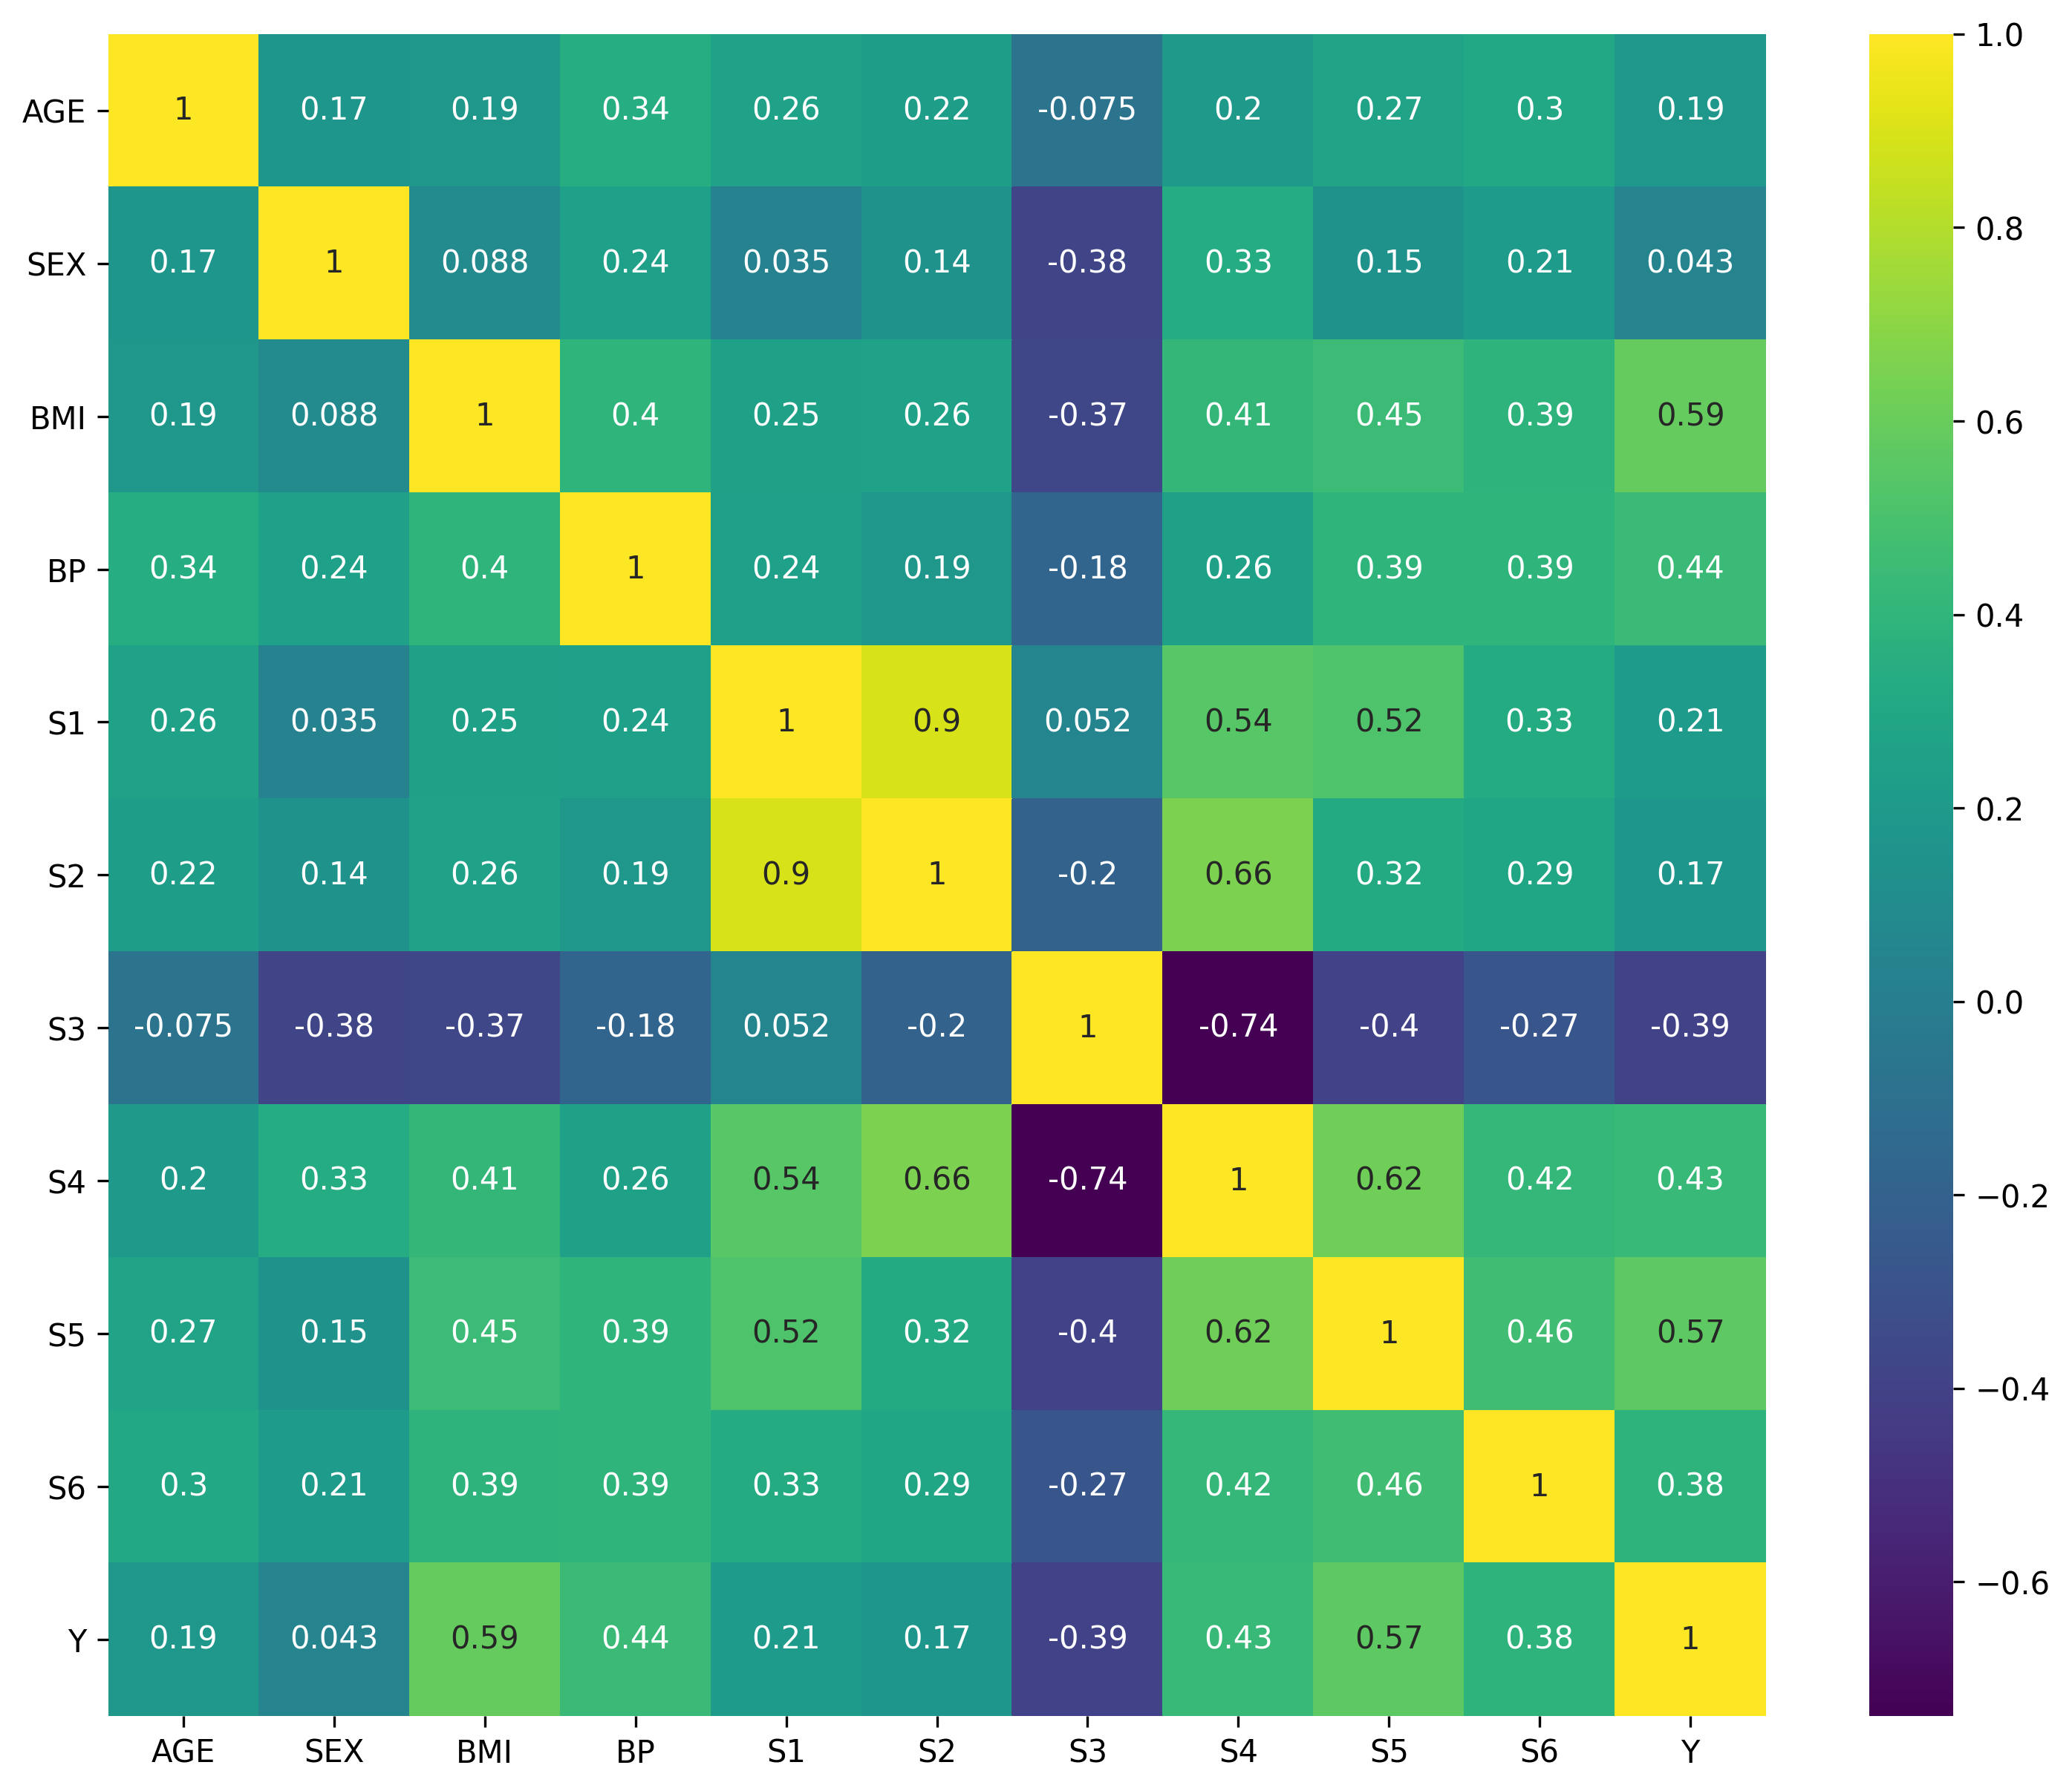
\includegraphics[width=\textwidth]{Corr}
\caption{Biểu đồ hệ số tương quan} \label{fig2}
\end{figure}

Biểu đồ hệ số tương quan là công cụ giúp chúng ta có cái nhìn trực quan và rõ ràng hơn về sự tương tác của các thuộc tính với nhau thông qua hệ số tương quan của những cặp thuộc tính. 

Hệ số tương quan là một thước đo thống kê về độ mạnh yếu của mối quan hệ giữa các chuyển động tương đối của hai biến. Có một số loại hệ số tương quan, nhưng loại phổ biến nhất là hệ số tương quan Pearson (R). Hệ số này chỉ ra độ mạnh và hướng của quan hệ tuyến tính giữa hai biến và có giá trị từ -1.0 đến 1.0. Trong đó, nếu:
\begin{itemize}
\item Hệ số tương quan dương: cho thấy mối quan hệ đồng biến hoặc tương quan dương (đồng biến tuyệt đối khi giá trị bằng 1.0).
\item Hệ số tương quan bằng 0: không có quan hệ tuyến tính giữa hai biến.
\item Hệ số tương quan âm: các biến có mối quan hệ nghịch biến hoặc tương quan âm (nghịch biến tuyệt đối khi giá trị bằng -1.0).
\end{itemize}

Qua biểu đồ hệ số tương quan, chúng tôi nhận thấy thuộc tính Y tương quan mạnh với thuộc tính BMI và S5 với hệ số tương quan lần lượt là 0.59 và 0.57. 

Hai thuộc tính tương quan dương rất mạnh với nhau là thuộc tính S1 và S2 với hệ số tương quan là 0.9, một số thuộc tính cũng có độ tương quan cao như S2 và S4 (coef = 0.66), S4 và S5 (coef = 0.62),...

Thuộc tính S3 có quan hệ nghịch biến (tương quan âm) với các thuộc tính còn lại, trong đó tương quan âm mạnh nhất là với thuộc tính S4 với hệ số tương quan là -0.74.
Điều này có thể ảnh hưởng không tốt đến các mô hình hồi quy, đặc biệt là mô hình hồi quy đa biến.

\vspace{0.5cm}
\textbf{Phân phối giá trị của thuộc tính Y}
\begin{figure}[H]
\centering
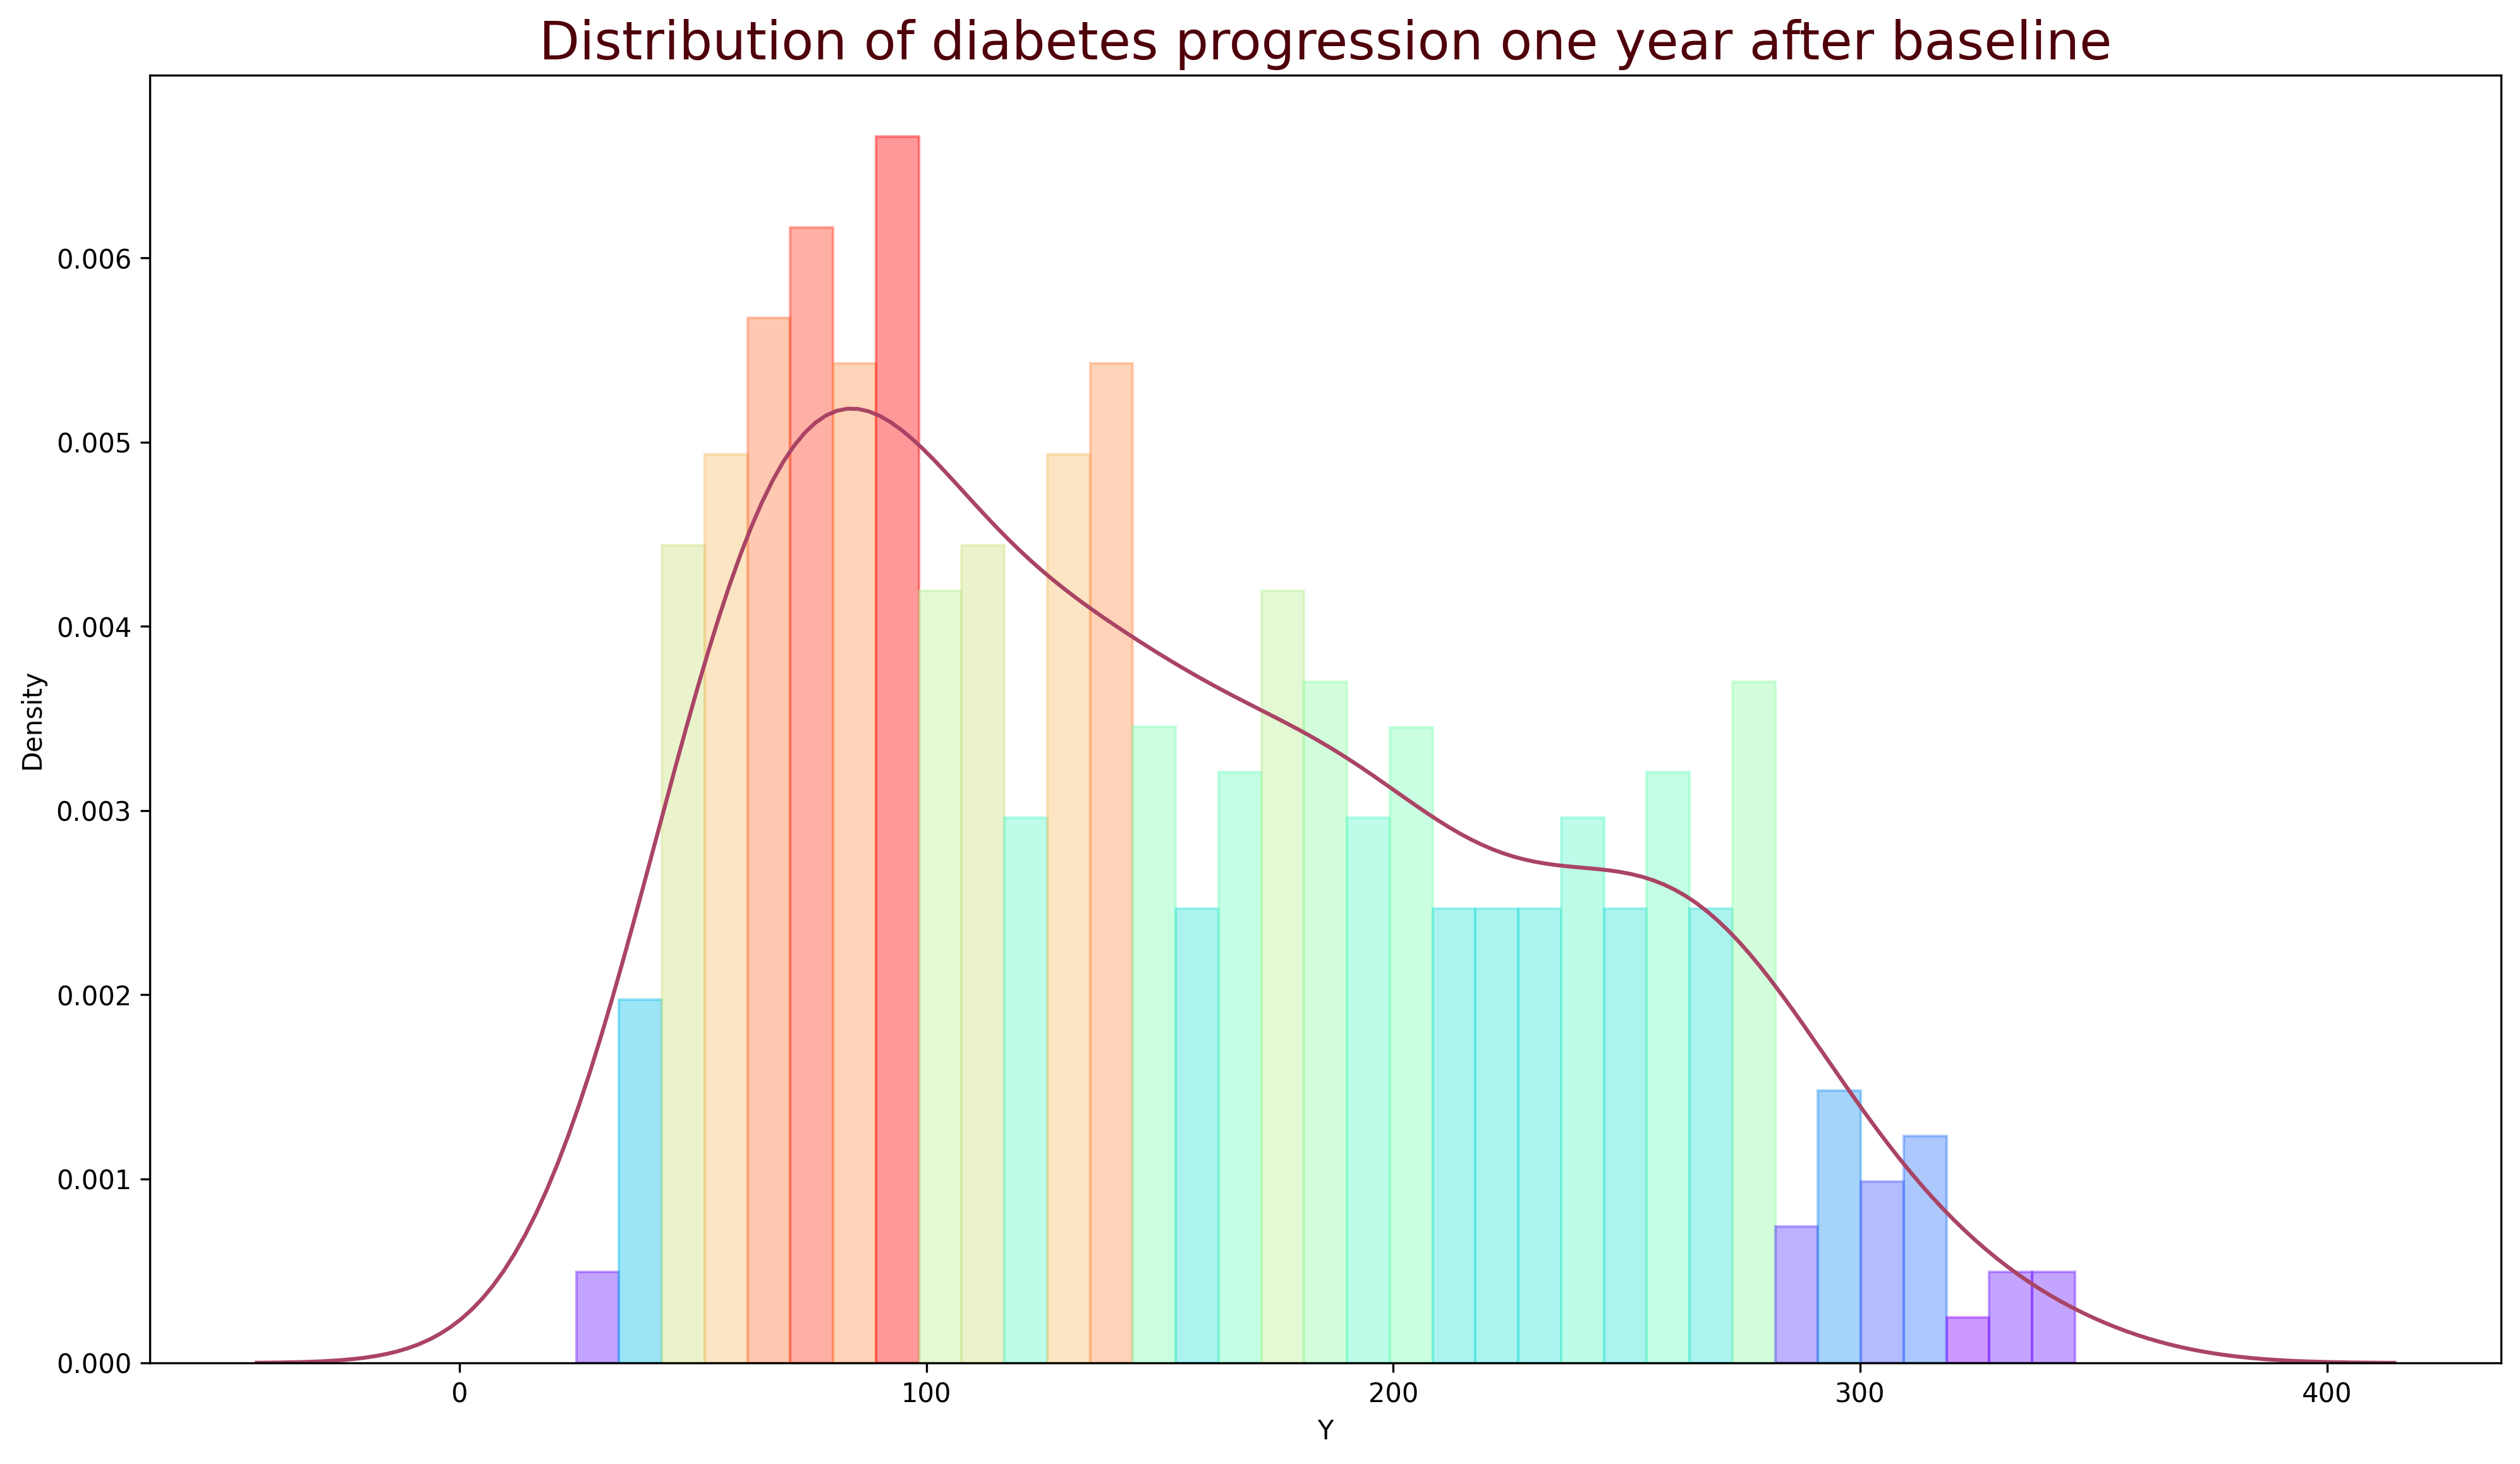
\includegraphics[width=\textwidth]{Dist_Y}
\caption{Biểu đồ phân phối giá trị thuộc tính Y} \label{fig2}
\end{figure}

Phân bố chỉ số tiến triển của các bệnh nhân có sự biến động nhưng không lớn, tiến triển bệnh tập trung nhiều từ chỉ số 100 trở lại. Hình dạng của biểu đồ bị lệch về bên trái cho thấy nhiều bệnh nhân đang ở giai đoạn đầu của bệnh đái tháo đường.


\vspace{0.5cm}
\textbf{Phân phối giá trị của thuộc tính BMI}

\begin{figure}[H]
\centering
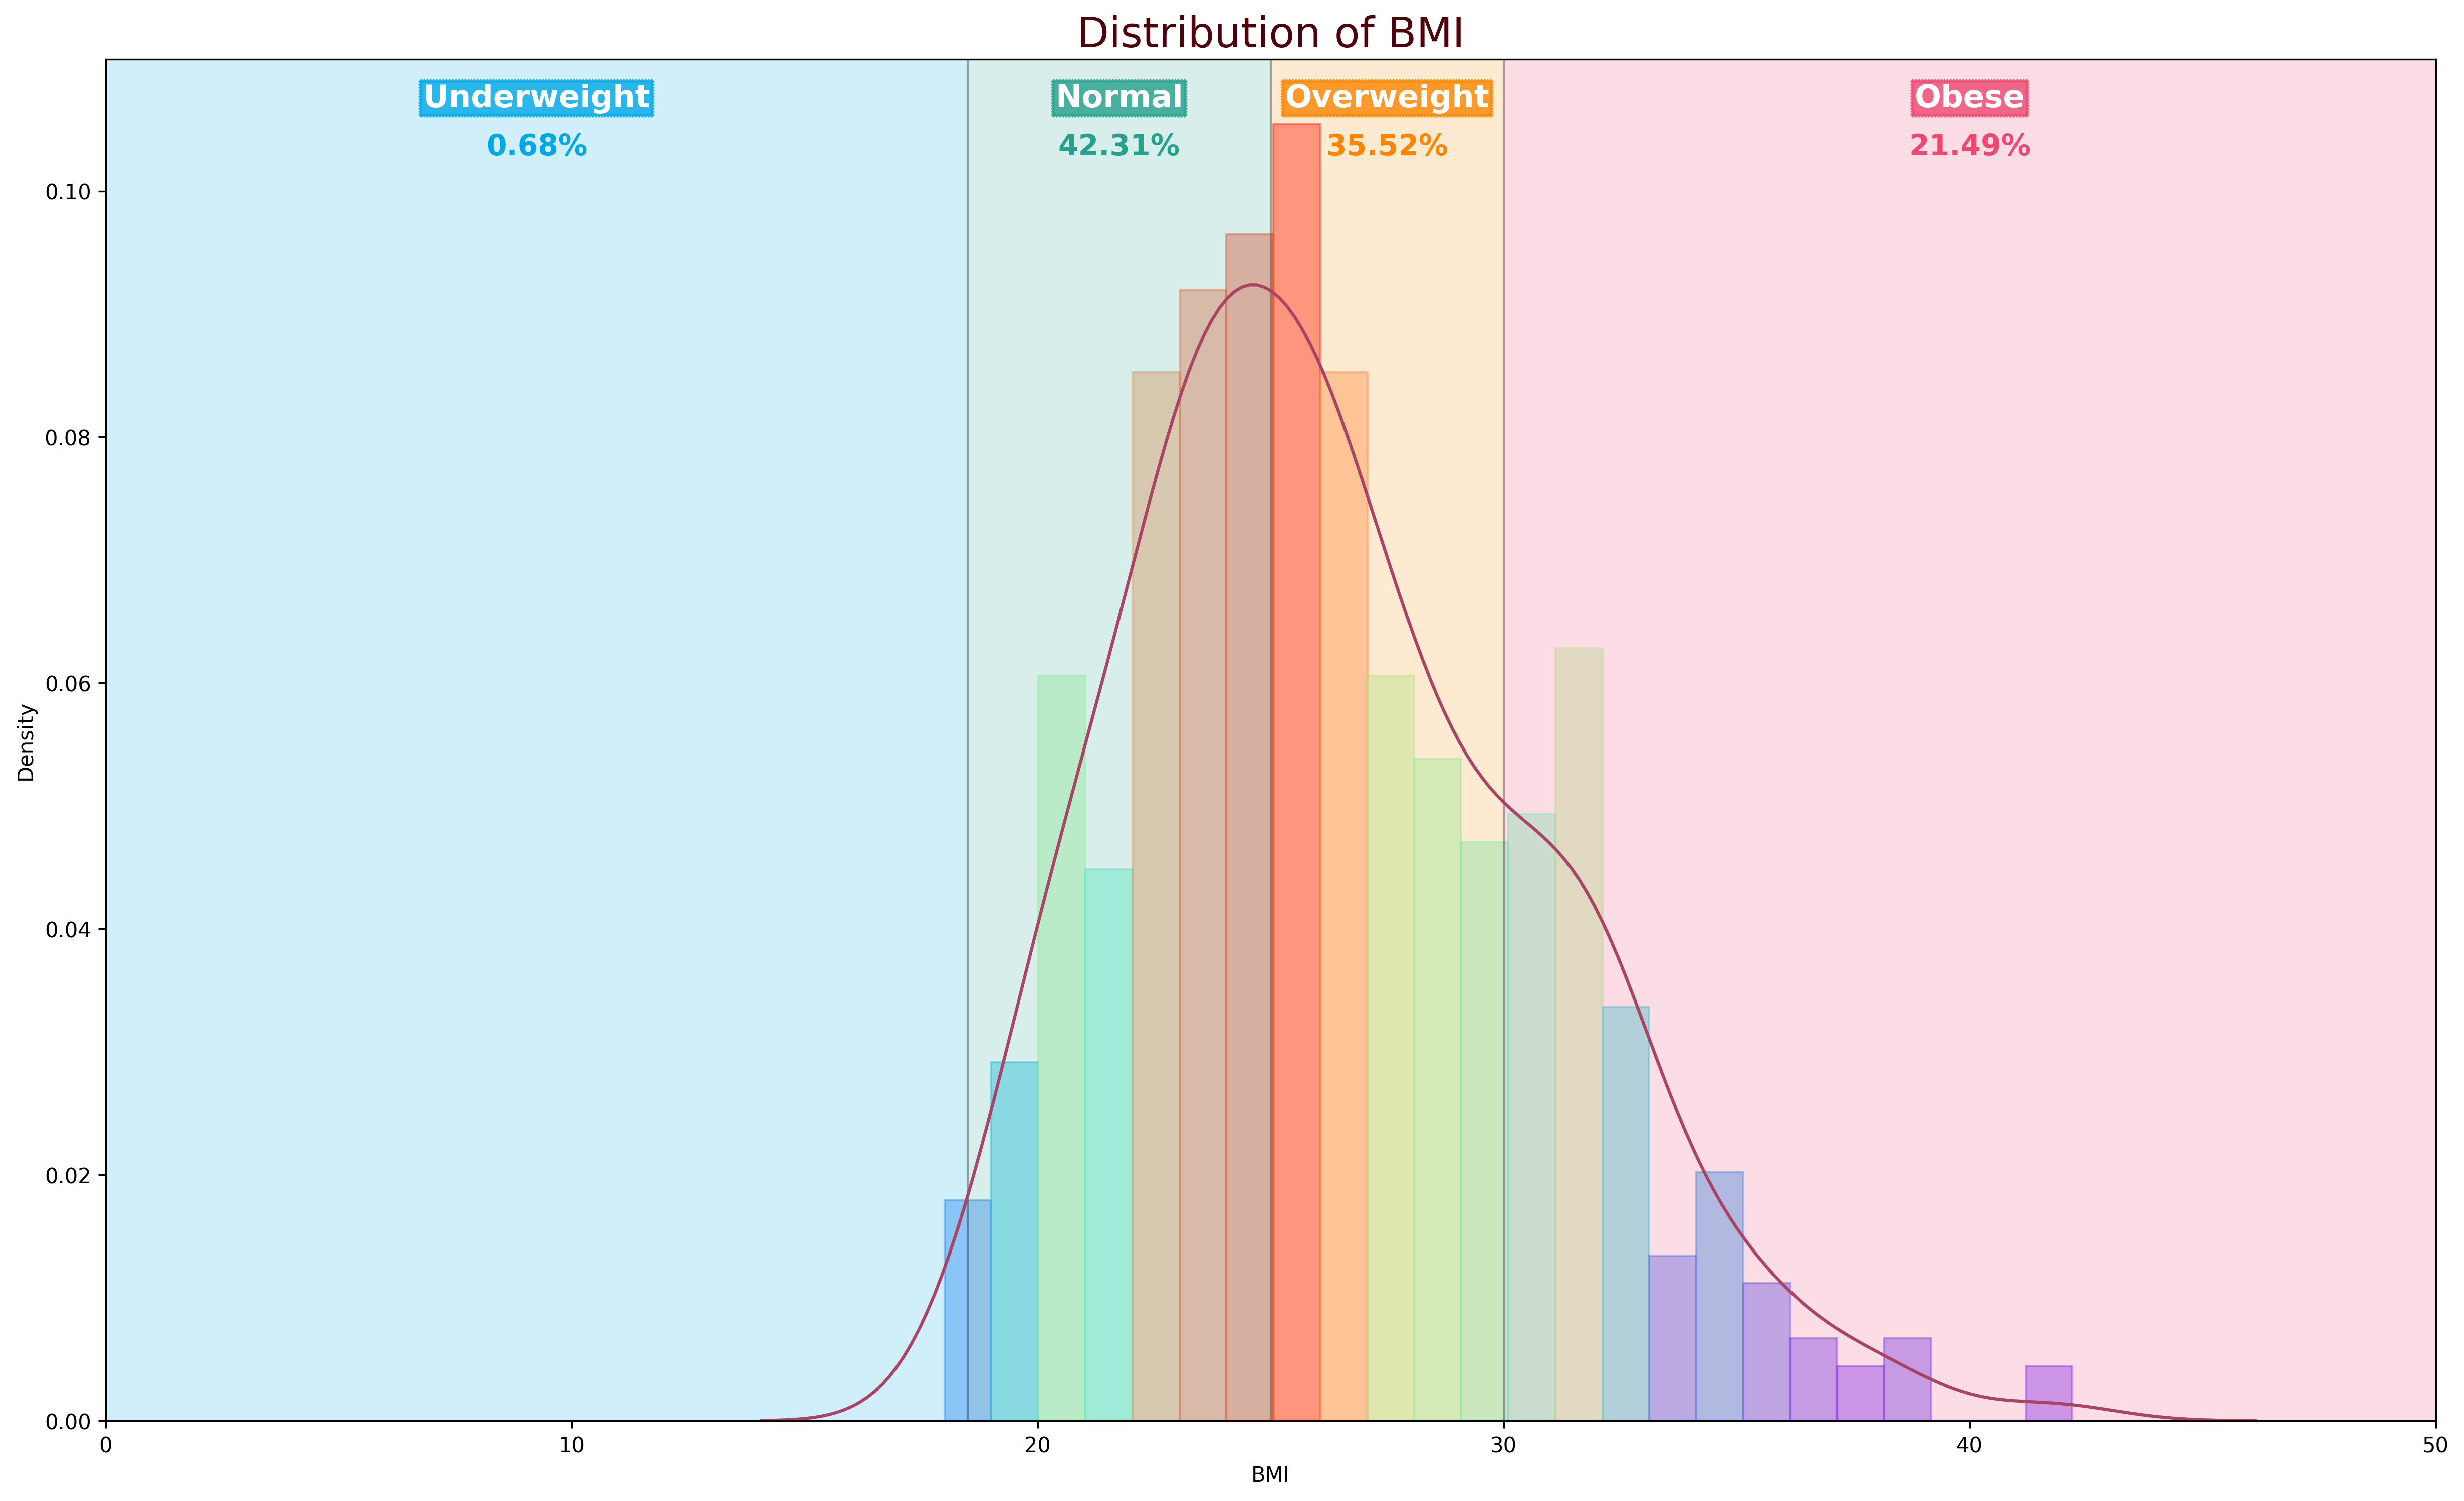
\includegraphics[width=\textwidth]{Dist_BMI}
\caption{Biểu đồ phân phối giá trị thuộc tính BMI} \label{fig2}
\end{figure}

Dựa vào biểu đồ phân phối chỉ số BMI, đa số các bệnh nhân có chỉ số khối cơ thể ở mức bình thường và thừa cân. Phân bố các điểm dữ liệu xấp xỉ về dạng phân phối chuẩn.

Chỉ có khoảng 0.68\% bệnh nhân được phân vào mức gầy và thiếu cân nhưng có tới 21,49\% bệnh nhân được xác định là béo phì. Đây là tình trạng rất phổ biến tại các quốc gia phát triển, trong trường hợp này là nước Mỹ, nơi các bệnh nhân được lấy mẫu.


\pagebreak
\section{Tiền xử lý dữ liệu}
\subsection{Xử lý ngoại lệ}

\begin{figure}[H]
\centering
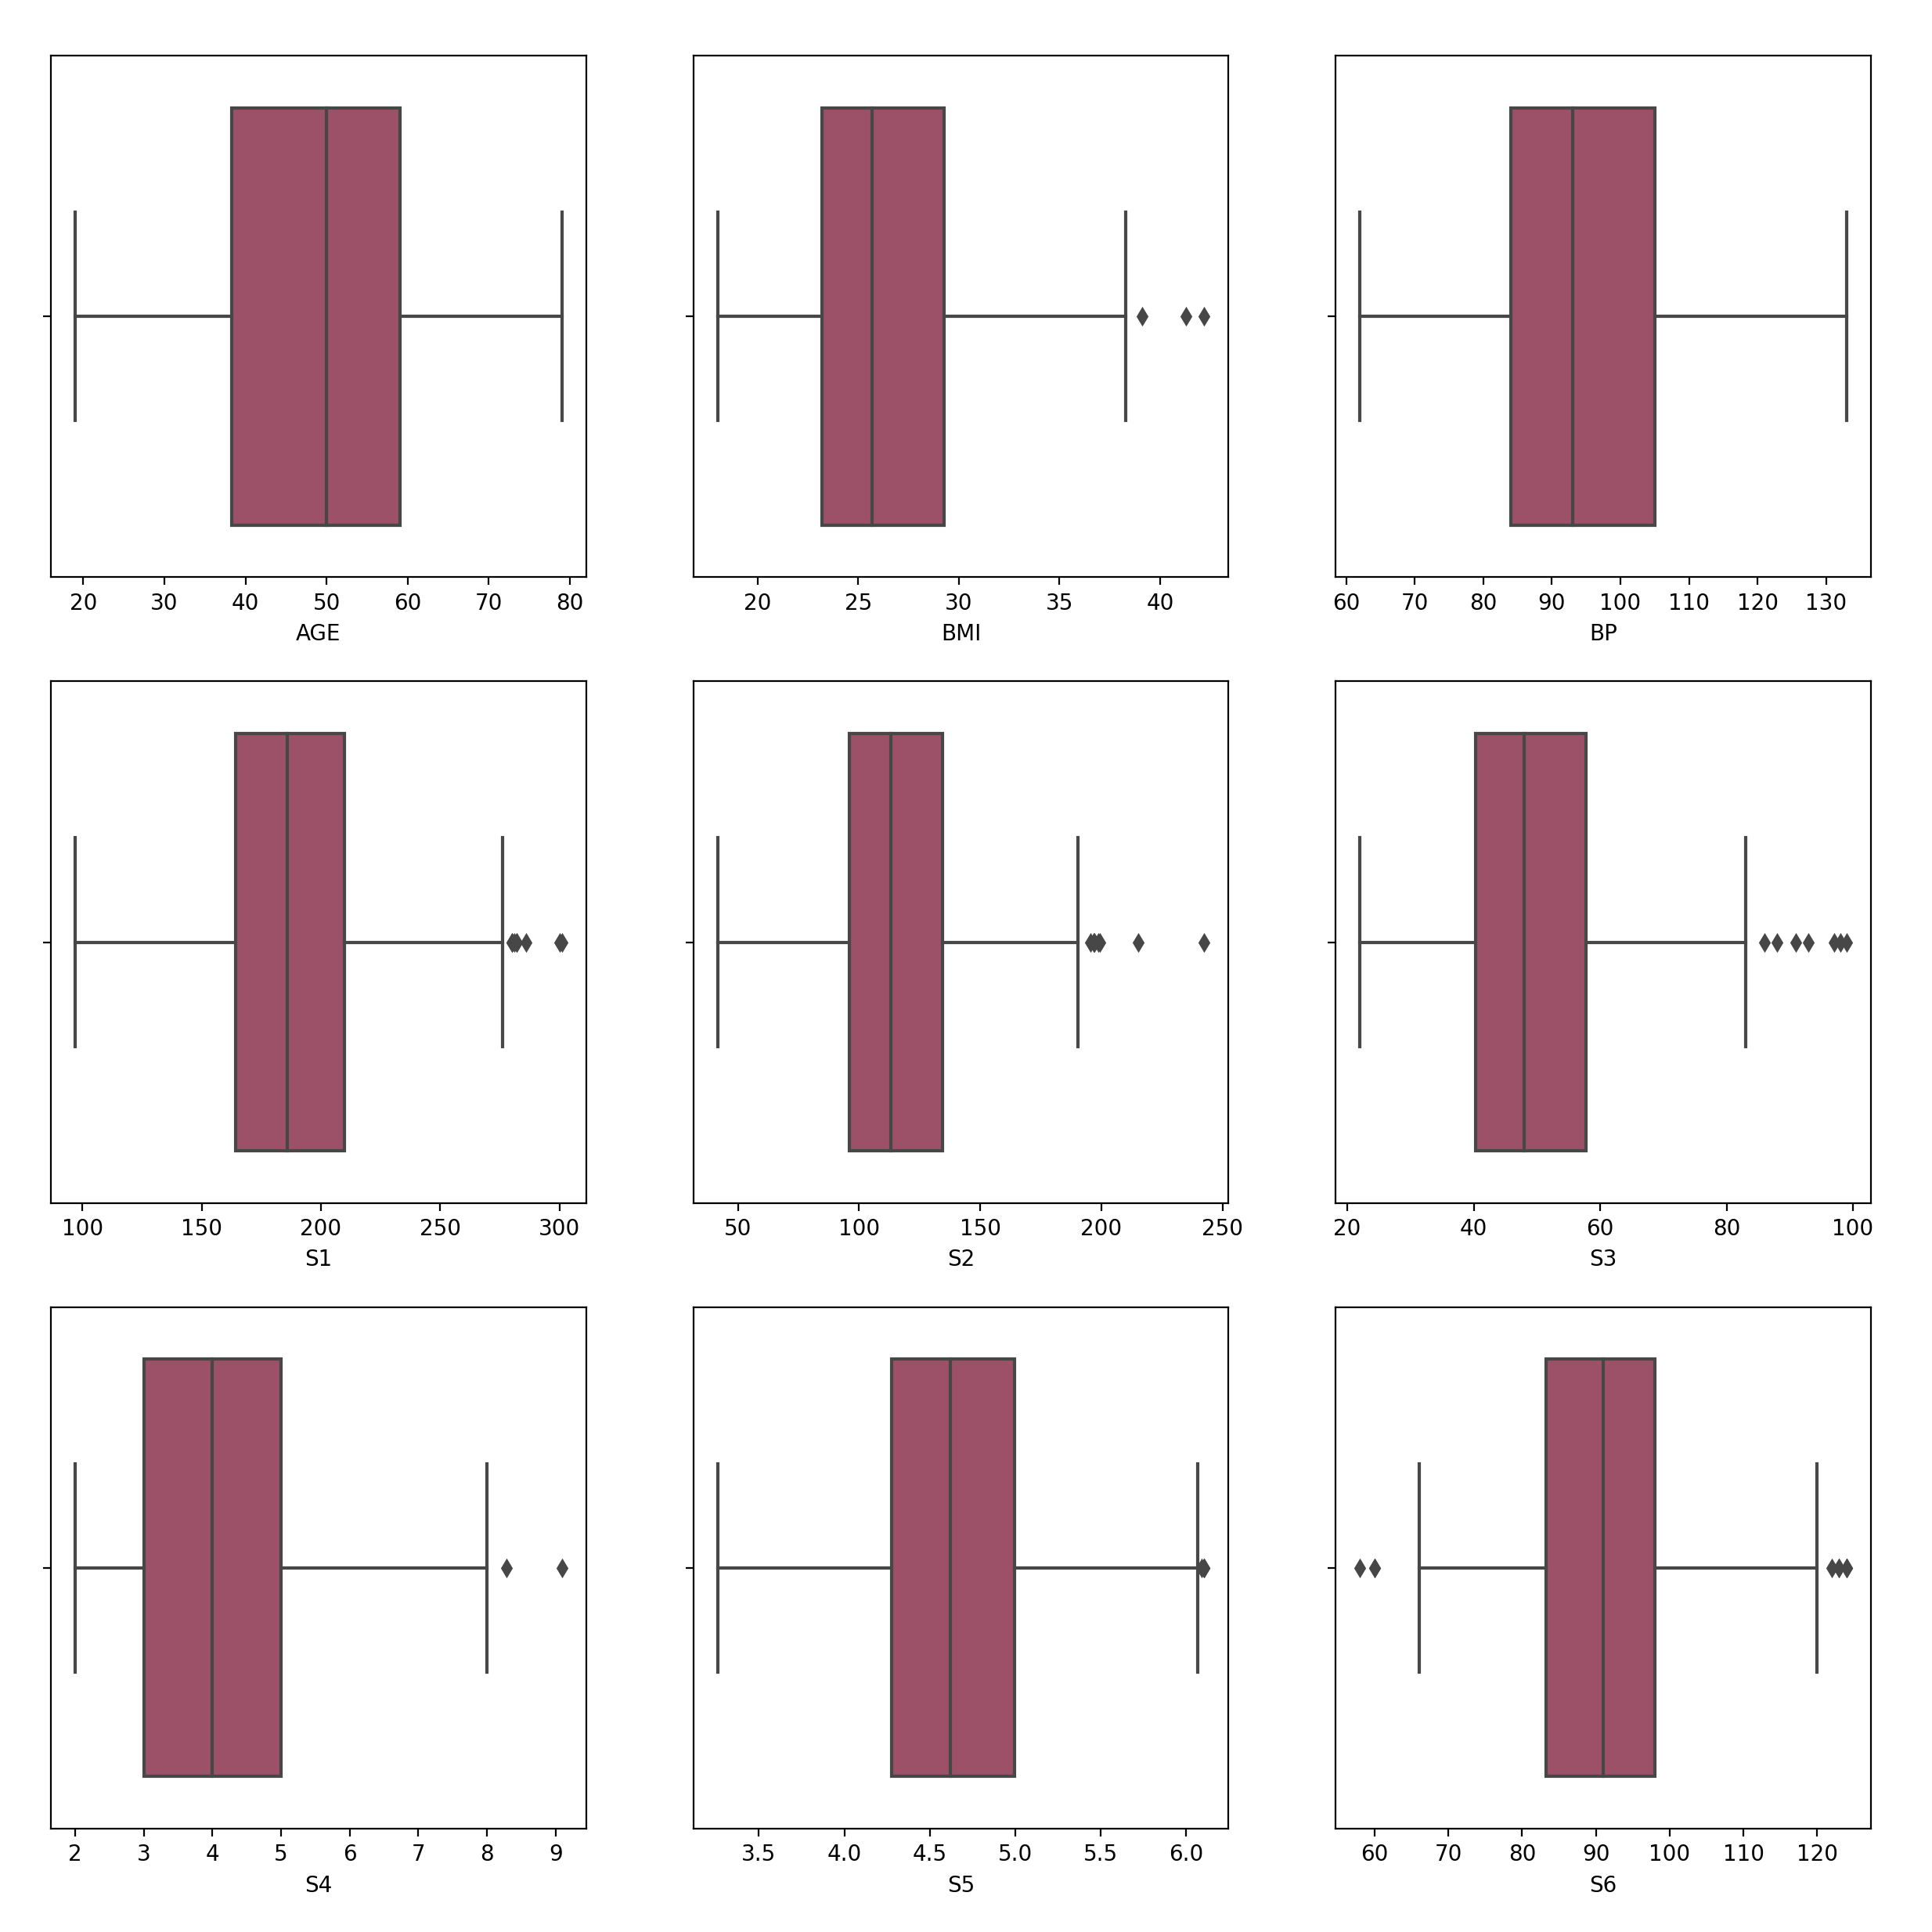
\includegraphics[width=\textwidth]{box}
\caption{Biểu đồ hộp của các thuộc tính định lượng} \label{fig2}
\end{figure}

Trong quá trình xử lý dữ liệu ngoại lệ (outlier), biểu đồ hộp là một công cụ quan trọng giúp chúng ta thấy rõ được các outlier cần được xử lý. Đặc điểm của biểu đồ hộp là thể hiện được các đại lượng quan trọng của một thuộc tính, bao gồm giá trị nhỏ nhất (min), giá trị lớn nhất (max), tứ phân vị (quartile), khoảng biến thiên tứ phân vị (Interquartile Range) một cách trực quan, dễ hiểu. Từ đó, nó cho thấy những điểm dữ liệu bất thường nằm xa phạm vi các giá trị trên.

Dựa vào biểu đồ hộp của các thuộc tính định lượng có thể dễ nhận thấy ở các thuộc tính BMI, S1, S2, S3, S4, S5 và S6 xuất hiện những điểm dữ liệu bất thường. Để loại bỏ chúng, chúng tôi dựa vào công thức rút ra từ biểu đồ hộp và tiến hành như sau:
\begin{itemize}
\item Đối với outlier bên trái biểu đồ hộp: Loại bỏ các điểm dữ liệu nhỏ hơn $Q1-1.5*IQR$
\item Đối với outlier bên phải biểu đồ hộp: Loại bỏ các điểm dữ liệu lớn hơn $Q3+1.5*IQR$
\end{itemize}
Trong đó: Q1 là tứ phân vị thứ 25, Q3 là tứ phân vị thứ 75, IQR là hiệu của Q3 và Q1. Sau đây là so sánh biểu đồ phân tán của các thuộc tính trước và sau khi loại bỏ ngoại lệ.

\begin{figure}[H]
\centering
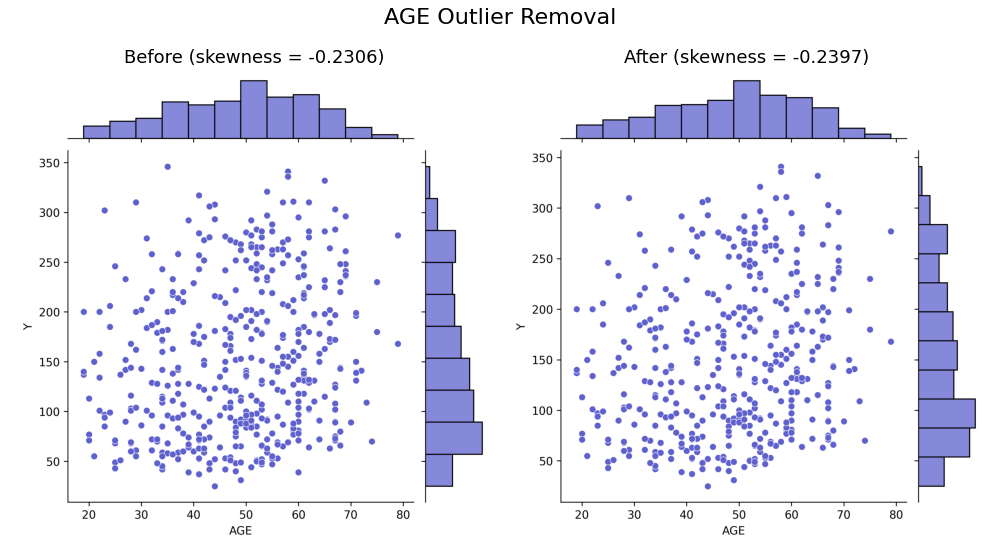
\includegraphics[width=0.9\textwidth]{AGEOR}
\caption{Biểu đồ phân tán của thuộc tính AGE so với Y trước và sau khi tiền xử lý} \label{fig2}
\vspace{0.5cm}
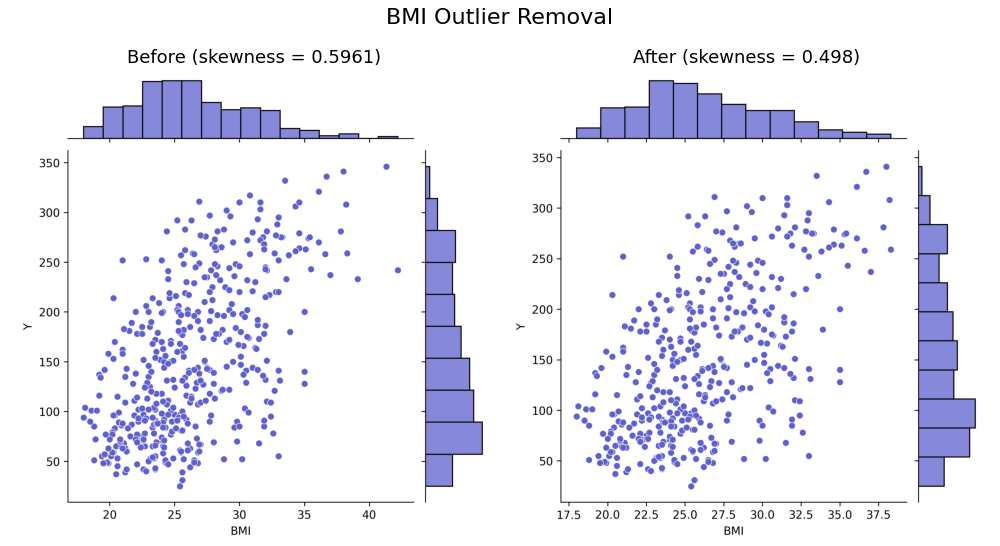
\includegraphics[width=0.9\textwidth]{BMIOR}
\caption{Biểu đồ phân tán của thuộc tính BMI so với Y trước và sau khi tiền xử lý} \label{fig2}
\end{figure}

\begin{figure}[H]
\centering
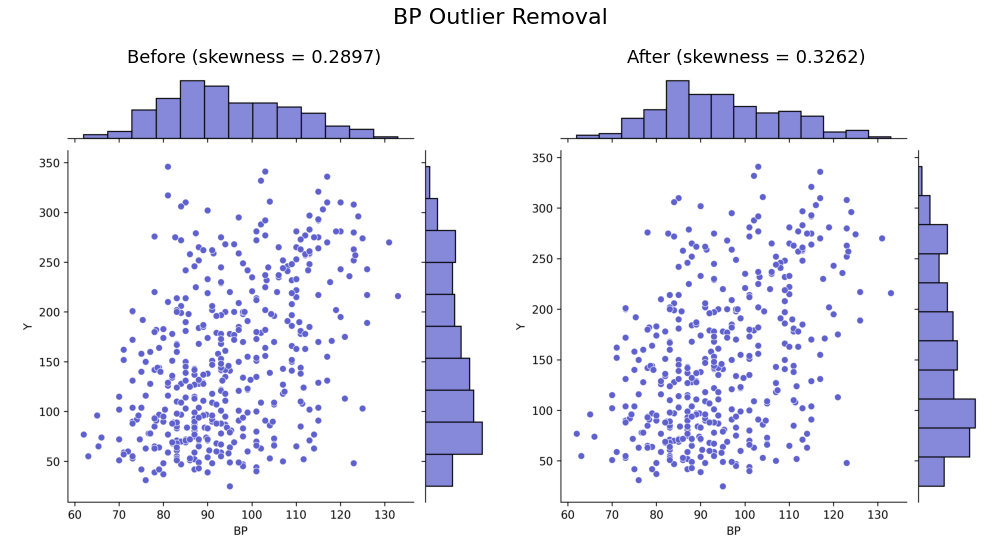
\includegraphics[width=0.9\textwidth]{BPOR}
\caption{Biểu đồ phân tán của thuộc tính BP so với Y trước và sau khi tiền xử lý} \label{fig2}
\vspace{0.5cm}
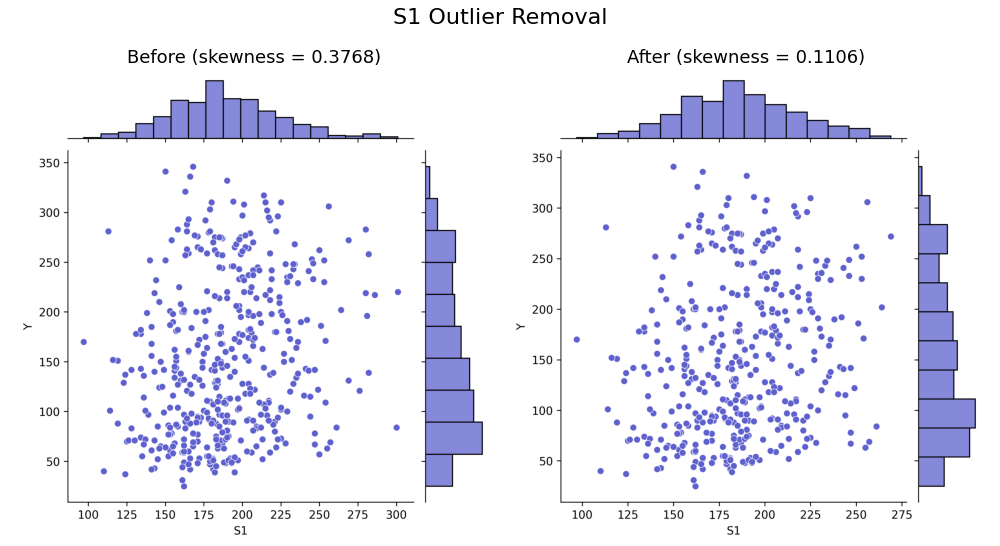
\includegraphics[width=0.9\textwidth]{S1OR}
\caption{Biểu đồ phân tán của thuộc tính S1 so với Y trước và sau khi tiền xử lý} \label{fig2}
\vspace{0.5cm}
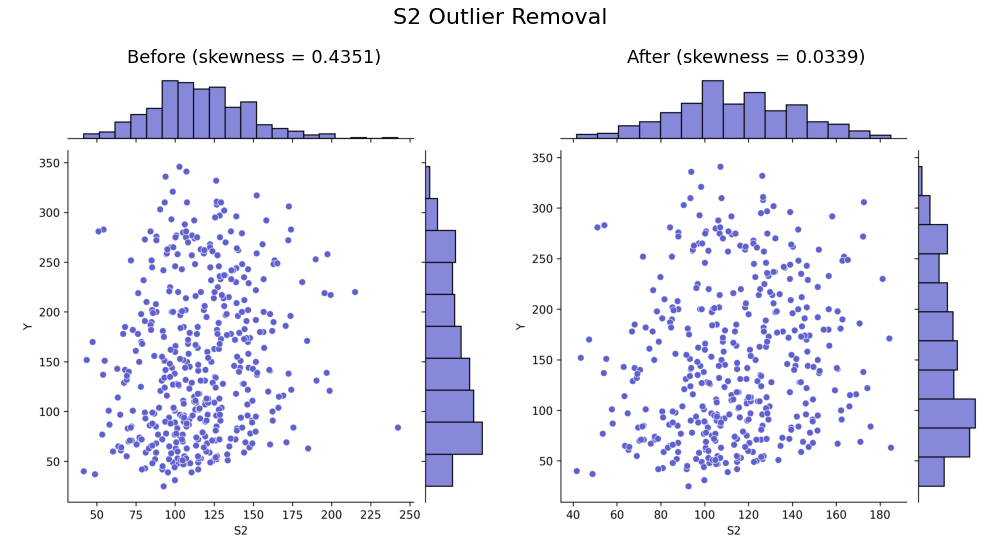
\includegraphics[width=0.9\textwidth]{S2OR}
\caption{Biểu đồ phân tán của thuộc tính S2 so với Y trước và sau khi tiền xử lý} \label{fig2}
\end{figure}

\begin{figure}[H]
\centering
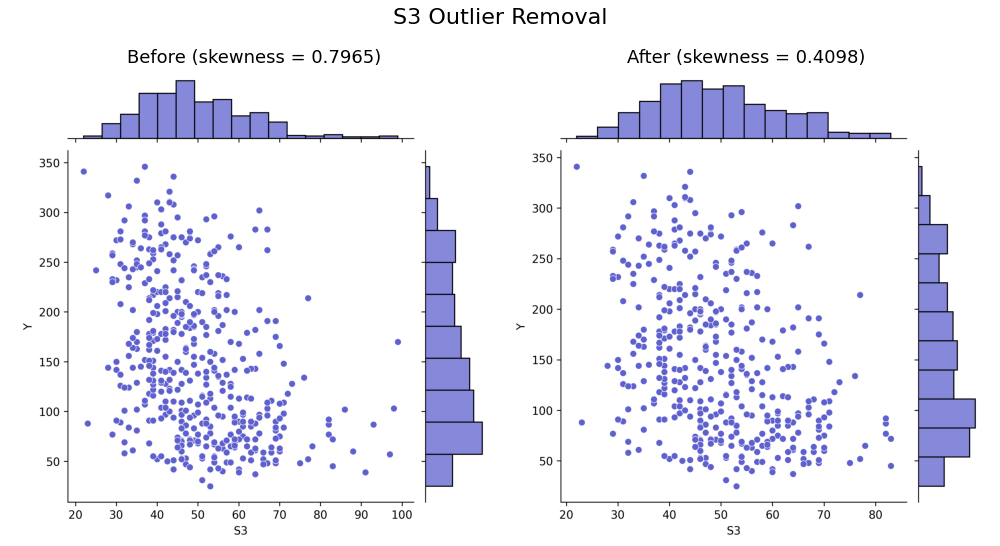
\includegraphics[width=0.9\textwidth]{S3OR}
\caption{Biểu đồ phân tán của thuộc tính S3 so với Y trước và sau khi tiền xử lý} \label{fig2}
\vspace{0.5cm}
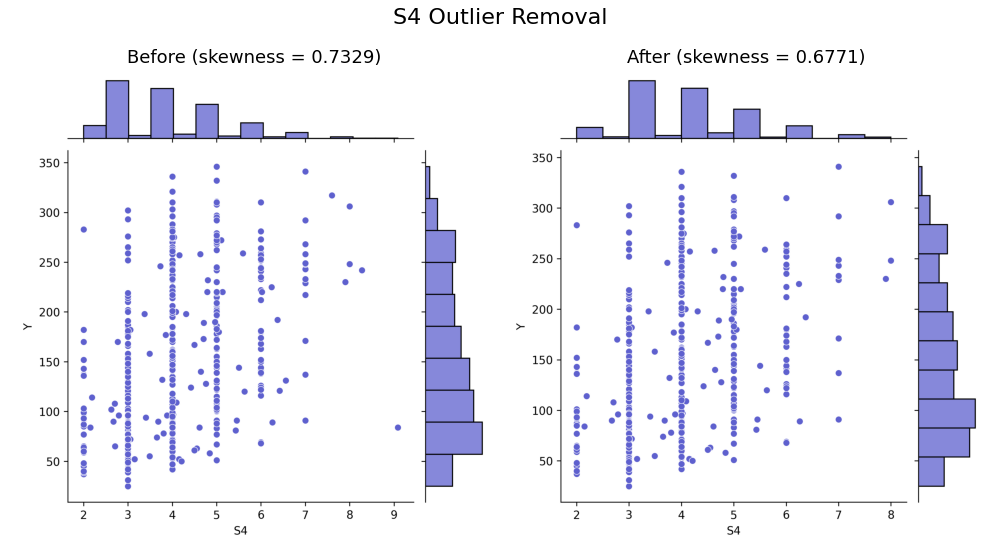
\includegraphics[width=0.9\textwidth]{S4OR}
\caption{Biểu đồ phân tán của thuộc tính S4 so với Y trước và sau khi tiền xử lý} \label{fig2}
\vspace{0.5cm}
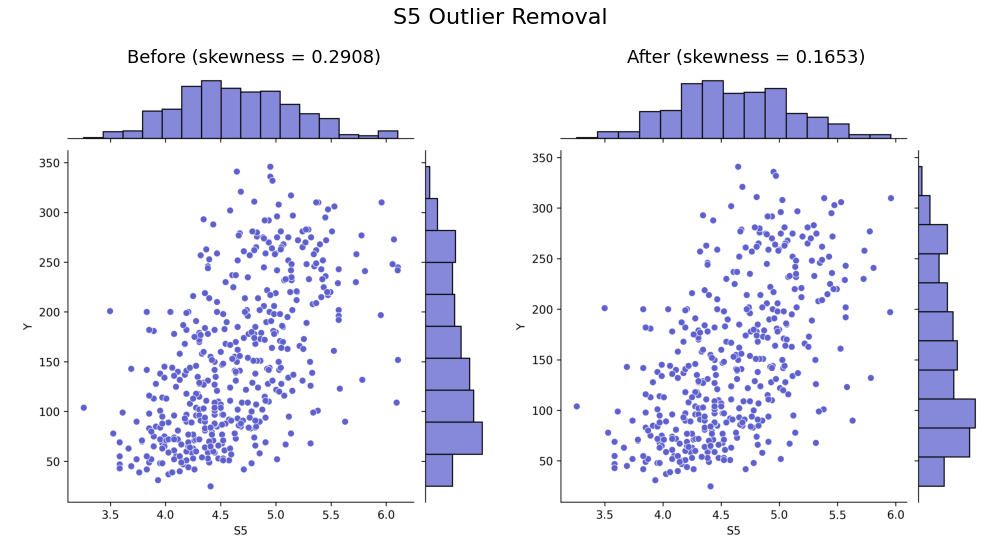
\includegraphics[width=0.9\textwidth]{S5OR}
\caption{Biểu đồ phân tán của thuộc tính S5 so với Y trước và sau khi tiền xử lý} \label{fig2}
\end{figure}

\begin{figure}[H]
\centering
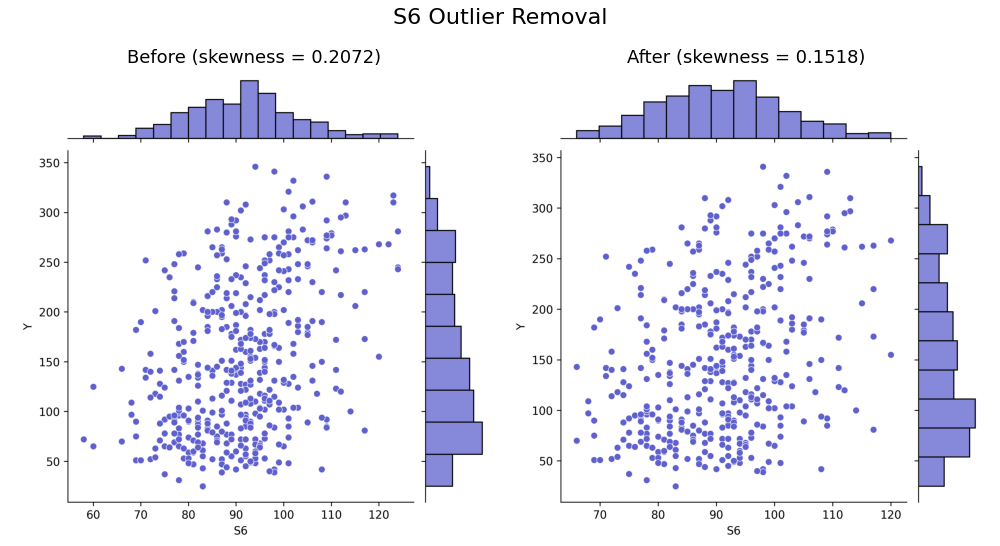
\includegraphics[width=0.9\textwidth]{S6OR}
\caption{Biểu đồ phân tán của thuộc tính S6 so với Y trước và sau khi tiền xử lý} \label{fig2}
\end{figure}

\subsection{Phân chia tập train và test}

Ở mỗi bộ dữ liệu trước và sau khi tiền xử lý, chúng tôi tiến hành chia dữ liệu thành hai tập train và test để phục vụ việc phân tích hồi quy và so sánh kết quả mô hình. Việc chia train test giúp các mô hình tránh overfitting và giúp đánh giá hiệu suất mô hình hiệu quả hơn. Sử dụng hàm createDataPartition có sẵn trong R, các tập train và test được chia theo tỉ lệ 8:2. Sau đây là kích thước của các tập dữ liệu.

\begin{table}
	\setlength{\tabcolsep}{0.5em}
	\renewcommand{\arraystretch}{1.4}
	\begin{center}
		\caption{Kích thước của các tập dữ liệu sau khi chia train test}\label{tab3}
		\begin{tabular}{|c|c|c|}
			\hline
			Bộ dữ liệu&Kích thước tập train&Kích thước tập test\\
			\hline
			Trước khi tiền xử lý&355&87\\
			\hline
			Sau khi tiền xử lý&327&80\\
			\hline
		\end{tabular}			
	\end{center}
\end{table}

\section{Phân tích hồi quy}

\subsection{Tổng quan về Phân tích Hồi quy (Regression Analysis)}
Phân tích hồi quy là một phương pháp thống kê mạnh mẽ cho phép xem xét mối tương quan giữa các biến số trong việc đo lường. Có nhiều loại phân tích hồi quy khác nhau nhưng chúng tựu chung đều tập trung vào việc đánh giá sự ảnh hưởng của các biến số độc lập lên một biến phụ thuộc.

Đây cũng là một phương pháp đáng tin cậy để xác định xem liệu biến số nào có ảnh hưởng đến bài toán đo lường (topic of interest). Quá trình thực hiện hồi quy cho phép xác định được yếu tố nào đáng quan tâm nhất và những yếu tố nào có thể bỏ qua, hay sự ảnh hưởng, tương tác lẫn nhau của các yếu tố.

Để hiểu một cách đầy đủ về phương pháp phân tích hồi quy, trước hết cần phải nắm vững một vài thuật ngữ sau:
\begin{itemize}
	\item \textbf{Biến phụ thuộc}: yếu tố chính cần được ước lượng, hiểu rõ và dự đoán 
	\item \textbf{Biến độc lập}: những yếu tố được giả thiết rằng có ảnh hưởng đến biến phụ thuộc
\end{itemize}

\subsection{Phân tích ảnh hưởng của các yếu tố và tương tác giữa các yếu tố}
Sau đây chúng tôi lần lượt phân tích những ảnh hưởng và tương tác giữa các yếu tố đến thuộc tính Y trên tập huấn luyện trước và sau khi xử lý, sử dụng bảng phân tích phương sai hai chiều (Two Way ANOVA). Để thuận tiện, chúng tôi xin viết tắt \textit{train} để chỉ tập huấn luyện trước khi tiền xử lý, \textit{train\_p} để chỉ tập huấn luyện sau khi tiền xử lý.
\subsubsection{Phân tích ảnh hưởng của các yếu tố khi không có tương tác}:

\vspace{0.5cm}
\textbf{Dữ liệu trước khi tiền xử lý:}
\begin{center}
\begin{tabular}{c}
\begin{lstlisting}[language=R]
av <- aov(Y~.,data=train)
summary(av)
\end{lstlisting}
\end{tabular}
\end{center}
\hrule

\begin{lcverbatim}
          Df  Sum Sq Mean Sq F value   Pr(>F)    
AGE           1   85855   85855  28.653 1.58e-07 ***
SEX           1     252     252   0.084    0.772    
BMI           1  591812  591812 197.514  < 2e-16 ***
BP            1  104605  104605  34.911 8.30e-09 ***
S1            1    5132    5132   1.713    0.191    
S2            1    4662    4662   1.556    0.213    
S3            1  173465  173465  57.893 2.68e-13 ***
S4            1    1210    1210   0.404    0.526    
S5            1   50637   50637  16.900 4.93e-05 ***
S6            1    4458    4458   1.488    0.223    
Residuals   344 1030730    2996                     
---
Signif. codes:  0 ‘***’ 0.001 ‘**’ 0.01 ‘*’ 0.05 ‘.’ 0.1 ‘ ’ 1
\end{lcverbatim}


\hrule
\vspace{0.5cm}

\textbf{Dữ liệu sau khi tiền xử lý:}
\begin{center}
\begin{tabular}{c}
\begin{lstlisting}[language=R]
av <- aov(Y~.,data=train_p)
summary(av)
\end{lstlisting}
\end{tabular}
\end{center}
\hrule
\begin{lcverbatim}
             Df Sum Sq Mean Sq F value   Pr(>F)    
AGE           1  70622   70622  24.021 1.53e-06 ***
SEX           1      2       2   0.001  0.98169    
BMI           1 464953  464953 158.147  < 2e-16 ***
BP            1  91331   91331  31.065 5.35e-08 ***
S1            1   1124    1124   0.382  0.53685    
S2            1    746     746   0.254  0.61481    
S3            1 223592  223592  76.052  < 2e-16 ***
S4            1    358     358   0.122  0.72744    
S5            1  20759   20759   7.061  0.00828 ** 
S6            1    661     661   0.225  0.63580    
Residuals   316 929043    2940                     
---
Signif. codes:  0 ‘***’ 0.001 ‘**’ 0.01 ‘*’ 0.05 ‘.’ 0.1 ‘ ’ 1
\end{lcverbatim}
\hrule
\vspace{0.5cm}

\textbf{Nhận xét:}
Qua bảng ANOVA, hai thuộc tính SEX và S4 đều cho giá tri p\_value lớn hơn các thuộc tính còn lại, lần lượt là 0.772 và 0.525 ở tập train, 0.98169 và 0.72744 ở tập train\_p. Các giá trị này đều lớn hơn mức ý nghĩa alpha 0.05, cho thấy khi không xảy ra tương tác thì 2 thuộc tính này không ảnh hưởng đến tiến triển bệnh tiểu đường (Y). Ngoài ra còn những yếu tố khác không ảnh hưởng tiến triển bệnh như S1, S2 và S6.

\subsubsection{Phân tích ảnh hưởng của các yếu tố khi có tương tác với SEX}:
\vspace{0.5cm}

\textbf{Dữ liệu trước khi tiền xử lý:}
\begin{center}
\begin{tabular}{c}
\begin{lstlisting}[language=R]
av <- aov(Y~(AGE+BMI+BP+S1+S2+S3+S5+S6)*SEX,data=train)
summary(av)
\end{lstlisting}
\end{tabular}
\end{center}
\hrule
\begin{lcverbatim}
             Df Sum Sq Mean Sq F value   Pr(>F)    
AGE           1  85855   85855  29.032 1.34e-07 ***
BMI           1 591789  591789 200.115  < 2e-16 ***
BP            1  98099   98099  33.172 1.90e-08 ***
S1            1   5402    5402   1.827 0.177416    
S2            1   7923    7923   2.679 0.102591    
S3            1 147757  147757  49.965 9.06e-12 ***
S5            1  47191   47191  15.958 7.96e-05 ***
S6            1   3657    3657   1.237 0.266911    
SEX           1  33132   33132  11.204 0.000909 ***
AGE:SEX       1  16983   16983   5.743 0.017101 *  
\end{lcverbatim}
\begin{lcverbatim}
BMI:SEX       1   9617    9617   3.252 0.072228 .  
BP:SEX        1   1313    1313   0.444 0.505624    
S1:SEX        1    106     106   0.036 0.850020    
S2:SEX        1   6128    6128   2.072 0.150940    
S3:SEX        1     74      74   0.025 0.874516    
S5:SEX        1    776     776   0.262 0.608866    
S6:SEX        1    425     425   0.144 0.704953    
Residuals   337 996590    2957                     
---
Signif. codes:  0 ‘***’ 0.001 ‘**’ 0.01 ‘*’ 0.05 ‘.’ 0.1 ‘ ’ 1
\end{lcverbatim}
\hrule
\vspace{0.5cm}

\textbf{Dữ liệu sau khi tiền xử lý:}
\begin{center}
\begin{tabular}{c}
\begin{lstlisting}[language=R]
av <- aov(Y~(AGE+BMI+BP+S1+S2+S3+S5+S6)*SEX,data=train_p)
summary(av)
\end{lstlisting}
\end{tabular}
\end{center}
\hrule
\begin{lcverbatim}
             Df Sum Sq Mean Sq F value   Pr(>F)    
AGE           1  70622   70622  24.333 1.33e-06 ***
BMI           1 464743  464743 160.132  < 2e-16 ***
BP            1  86284   86284  29.730 1.02e-07 ***
S1            1   1359    1359   0.468 0.494335    
S2            1   2053    2053   0.707 0.401000    
S3            1 192796  192796  66.430 9.13e-15 ***
S5            1  22091   22091   7.612 0.006145 ** 
S6            1    369     369   0.127 0.721790    
SEX           1  32870   32870  11.326 0.000861 ***
AGE:SEX       1  18617   18617   6.415 0.011813 *  
BMI:SEX       1   6800    6800   2.343 0.126872    
BP:SEX        1    519     519   0.179 0.672724    
S1:SEX        1    614     614   0.212 0.645764    
S2:SEX        1   1687    1687   0.581 0.446379    
S3:SEX        1   2718    2718   0.936 0.333951    
S5:SEX        1    157     157   0.054 0.816196    
S6:SEX        1   2096    2096   0.722 0.396099    
Residuals   309 896796    2902                     
---
Signif. codes:  0 ‘***’ 0.001 ‘**’ 0.01 ‘*’ 0.05 ‘.’ 0.1 ‘ ’ 1
\end{lcverbatim}
\hrule
\vspace{0.5cm}

\textbf{Nhận xét:}
Khi xét trường hợp xảy ra tương tác giữa SEX với các yếu tố còn lại, thuộc tính SEX lúc này có giá trị  p\_value = 0.000909 trên tập train và p\_value = 0.000861 trên tập train\_p, đều nhỏ hơn 0.05 cho thấy ảnh hưởng đến tiến triển bệnh. Ngoài ra, tương tác AGE:SEX cũng cho thấy ảnh hưởng tới tiến triển bệnh với p\_value ở train và train\_p đều nhỏ hơn 0.05.


\subsubsection{Phân tích ảnh hưởng của các yếu tố khi có tương tác với S4}:
\vspace{0.5cm}

\textbf{Dữ liệu trước khi tiền xử lý:}
\begin{center}
\begin{tabular}{c}
\begin{lstlisting}[language=R]
av <- aov(Y~(AGE+BMI+BP+S1+S2+S3+S5+S6)*S4,data=train)
summary(av)
\end{lstlisting}
\end{tabular}
\end{center}
\hrule
\begin{lcverbatim}
             Df  Sum Sq Mean Sq F value   Pr(>F)    
AGE           1   85855   85855  27.968 2.22e-07 ***
BMI           1  591789  591789 192.779  < 2e-16 ***
BP            1   98099   98099  31.956 3.36e-08 ***
S1            1    5402    5402   1.760 0.185547    
S2            1    7923    7923   2.581 0.109082    
S3            1  147757  147757  48.133 2.05e-11 ***
S5            1   47191   47191  15.373 0.000107 ***
S6            1    3657    3657   1.191 0.275845    
S4            1     599     599   0.195 0.659068    
AGE:S4        1    5122    5122   1.669 0.197321    
BMI:S4        1   10028   10028   3.267 0.071591 .  
BP:S4         1     169     169   0.055 0.814705    
S1:S4         1    1218    1218   0.397 0.529180    
S2:S4         1     386     386   0.126 0.723111    
S3:S4         1     182     182   0.059 0.807668    
S5:S4         1    3702    3702   1.206 0.272916    
S6:S4         1    9221    9221   3.004 0.083984 .  
Residuals   337 1034516    3070                     
---
Signif. codes:  0 ‘***’ 0.001 ‘**’ 0.01 ‘*’ 0.05 ‘.’ 0.1 ‘ ’ 1
\end{lcverbatim}
\hrule
\vspace{0.5cm}

\textbf{Dữ liệu sau khi tiền xử lý:}
\begin{center}
\begin{tabular}{c}
\begin{lstlisting}[language=R]
av <- aov(Y~(AGE+BMI+BP+S1+S2+S3+S5+S6)*S4,data=train_p)
summary(av)
\end{lstlisting}
\end{tabular}
\end{center}
\hrule
\begin{lcverbatim}
             Df Sum Sq Mean Sq F value   Pr(>F)    
AGE           1  70622   70622  23.338 2.14e-06 ***
BMI           1 464743  464743 153.583  < 2e-16 ***
BP            1  86284   86284  28.514 1.81e-07 ***
S1            1   1359    1359   0.449  0.50329    
S2            1   2053    2053   0.678  0.41079    
S3            1 192796  192796  63.713 2.85e-14 ***
S5            1  22091   22091   7.301  0.00727 ** 
S6            1    369     369   0.122  0.72731    
S4            1    345     345   0.114  0.73595    
\end{lcverbatim}
\begin{lcverbatim}
AGE:S4        1   6128    6128   2.025  0.15574    
BMI:S4        1   5028    5028   1.662  0.19836    
BP:S4         1    268     268   0.088  0.76637    
S1:S4         1     14      14   0.005  0.94559    
S2:S4         1     10      10   0.003  0.95391    
S3:S4         1   1404    1404   0.464  0.49630    
S5:S4         1   4644    4644   1.535  0.21635    
S6:S4         1   9999    9999   3.304  0.07007 .  
Residuals   309 935035    3026                     
---
Signif. codes:  0 ‘***’ 0.001 ‘**’ 0.01 ‘*’ 0.05 ‘.’ 0.1 ‘ ’ 1
\end{lcverbatim}
\hrule
\vspace{0.5cm}

\textbf{Nhận xét:}
Bảng ANOVA cho thấy khi có tương tác giữa S4 với các yếu tố còn lại, thì S4 và các tương tác với nó đều không ảnh hưởng đến tiến triển bệnh với mức ý nghĩa 0.05.

\subsubsection{Phân tích ảnh hưởng của các yếu tố khi xảy ra tương tác}:
\vspace{0.5cm}

\textbf{Dữ liệu trước khi tiền xử lý:}
\begin{center}
\begin{tabular}{c}
\begin{lstlisting}[language=R]
av <- aov(Y~AGE*BMI*BP*S1*S2*S3*S5*S6+AGE*SEX,data=train)
summary(av)
\end{lstlisting}
\end{tabular}
\end{center}
\hrule
\begin{lcverbatim}
                       Df Sum Sq Mean Sq F value   Pr(>F)    
AGE                     1  85855   85855  28.663 5.59e-07 ***
BMI                     1 591789  591789 197.571  < 2e-16 ***
BP                      1  98099   98099  32.751 1.12e-07 ***
S1                      1   5402    5402   1.804 0.182355    
S2                      1   7923    7923   2.645 0.107038    
S3                      1 147757  147757  49.329 2.77e-10 ***
S5                      1  47191   47191  15.755 0.000137 ***
S6                      1   3657    3657   1.221 0.271858    
SEX                     1  33132   33132  11.061 0.001238 ** 
AGE:BMI                 1   9377    9377   3.131 0.079915 .  
AGE:BP                  1  11912   11912   3.977 0.048883 *  
BMI:BP                  1  21859   21859   7.298 0.008123 ** 
AGE:S1                  1      2       2   0.001 0.979064    
BMI:S1                  1  10422   10422   3.479 0.065098 .  
BP:S1                   1    208     208   0.069 0.792619    
AGE:S2                  1   8377    8377   2.797 0.097623 .  
BMI:S2                  1    523     523   0.175 0.676877    
BP:S2                   1     85      85   0.028 0.866446    
S1:S2                   1    469     469   0.157 0.693186    
AGE:S3                  1   1185    1185   0.396 0.530743    
\end{lcverbatim}
\begin{lcverbatim}
BMI:S3                  1     54      54   0.018 0.893198    
BP:S3                   1   2814    2814   0.939 0.334808    
S1:S3                   1   1916    1916   0.640 0.425734    
S2:S3                   1   3100    3100   1.035 0.311488    
AGE:S5                  1   7201    7201   2.404 0.124219    
BMI:S5                  1   2705    2705   0.903 0.344256    
BP:S5                   1   1357    1357   0.453 0.502542    
S1:S5                   1      1       1   0.000 0.984883    
S2:S5                   1   3635    3635   1.214 0.273279    
S3:S5                   1   1596    1596   0.533 0.467191    
AGE:S6                  1   3816    3816   1.274 0.261765    
BMI:S6                  1    890     890   0.297 0.586833    
BP:S6                   1   1259    1259   0.420 0.518276    
S1:S6                   1    895     895   0.299 0.585949    
S2:S6                   1    337     337   0.112 0.738034    
S3:S6                   1   5373    5373   1.794 0.183538    
S5:S6                   1    704     704   0.235 0.628842    
AGE:SEX                 1  18271   18271   6.100 0.015230 *  
AGE:BMI:BP              1   5803    5803   1.937 0.167085    
AGE:BMI:S1              1    968     968   0.323 0.570925    
AGE:BP:S1               1    583     583   0.195 0.660098    
BMI:BP:S1               1   1299    1299   0.434 0.511745    
AGE:BMI:S2              1   1138    1138   0.380 0.538982    
AGE:BP:S2               1   7179    7179   2.397 0.124789    
BMI:BP:S2               1   1414    1414   0.472 0.493618    
AGE:S1:S2               1    813     813   0.271 0.603555    
BMI:S1:S2               1   4960    4960   1.656 0.201177    
BP:S1:S2                1    124     124   0.041 0.839153    
AGE:BMI:S3              1    375     375   0.125 0.724075    
AGE:BP:S3               1   1591    1591   0.531 0.467810    
BMI:BP:S3               1    112     112   0.037 0.847059    
AGE:S1:S3               1   4336    4336   1.448 0.231792    
BMI:S1:S3               1   3601    3601   1.202 0.275545    
BP:S1:S3                1   3811    3811   1.272 0.262034    
AGE:S2:S3               1    343     343   0.114 0.735880    
BMI:S2:S3               1   1290    1290   0.431 0.513204    
BP:S2:S3                1    122     122   0.041 0.840332    
S1:S2:S3                1   2427    2427   0.810 0.370271    
AGE:BMI:S5              1   3688    3688   1.231 0.269844    
AGE:BP:S5               1  11160   11160   3.726 0.056441 .  
BMI:BP:S5               1   1309    1309   0.437 0.510087    
AGE:S1:S5               1   7515    7515   2.509 0.116400    
BMI:S1:S5               1  23173   23173   7.737 0.006480 ** 
BP:S1:S5                1   3932    3932   1.313 0.254694    
AGE:S2:S5               1    416     416   0.139 0.710188    
\end{lcverbatim}
\begin{lcverbatim}
BMI:S2:S5               1  11092   11092   3.703 0.057179 .  
BP:S2:S5                1     92      92   0.031 0.861310    
S1:S2:S5                1      9       9   0.003 0.957614    
AGE:S3:S5               1     13      13   0.004 0.948480    
BMI:S3:S5               1   3067    3067   1.024 0.314091    
BP:S3:S5                1   7129    7129   2.380 0.126074    
S1:S3:S5                1   1311    1311   0.438 0.509794    
S2:S3:S5                1     91      91   0.030 0.861746    
AGE:BMI:S6              1     20      20   0.007 0.934821    
AGE:BP:S6               1    758     758   0.253 0.615936    
BMI:BP:S6               1      1       1   0.000 0.988486    
AGE:S1:S6               1   7772    7772   2.595 0.110397    
BMI:S1:S6               1    128     128   0.043 0.836704    
BP:S1:S6                1   2193    2193   0.732 0.394283    
AGE:S2:S6               1    217     217   0.073 0.788285    
BMI:S2:S6               1      0       0   0.000 0.998612    
BP:S2:S6                1    207     207   0.069 0.793402    
S1:S2:S6                1   1446    1446   0.483 0.488765    
AGE:S3:S6               1    246     246   0.082 0.775180    
BMI:S3:S6               1   6598    6598   2.203 0.140947    
BP:S3:S6                1   9932    9932   3.316 0.071631 .  
S1:S3:S6                1    547     547   0.183 0.670023    
S2:S3:S6                1   3286    3286   1.097 0.297486    
AGE:S5:S6               1   5080    5080   1.696 0.195853    
BMI:S5:S6               1    327     327   0.109 0.741668    
BP:S5:S6                1    224     224   0.075 0.785122    
S1:S5:S6                1   1429    1429   0.477 0.491414    
S2:S5:S6                1   5046    5046   1.685 0.197343    
S3:S5:S6                1     25      25   0.008 0.927733    
AGE:BMI:BP:S1           1    174     174   0.058 0.810231    
AGE:BMI:BP:S2           1   4509    4509   1.506 0.222736    
AGE:BMI:S1:S2           1     56      56   0.019 0.891595    
AGE:BP:S1:S2            1    452     452   0.151 0.698440    
BMI:BP:S1:S2            1    202     202   0.067 0.795564    
AGE:BMI:BP:S3           1    694     694   0.232 0.631409    
AGE:BMI:S1:S3           1   3934    3934   1.313 0.254560    
AGE:BP:S1:S3            1    459     459   0.153 0.696184    
BMI:BP:S1:S3            1   3389    3389   1.131 0.290048    
AGE:BMI:S2:S3           1    473     473   0.158 0.691930    
AGE:BP:S2:S3            1   8922    8922   2.979 0.087493 .  
BMI:BP:S2:S3            1    299     299   0.100 0.752688    
AGE:S1:S2:S3            1   4464    4464   1.490 0.225069    
BMI:S1:S2:S3            1   8022    8022   2.678 0.104910    
BP:S1:S2:S3             1   1029    1029   0.344 0.559078    
AGE:BMI:BP:S5           1    210     210   0.070 0.791508    
\end{lcverbatim}
\begin{lcverbatim}
AGE:BMI:S1:S5           1   2977    2977   0.994 0.321222    
AGE:BP:S1:S5            1   2802    2802   0.936 0.335790    
BMI:BP:S1:S5            1   3643    3643   1.216 0.272745    
AGE:BMI:S2:S5           1     96      96   0.032 0.858016    
AGE:BP:S2:S5            1   4189    4189   1.399 0.239789    
BMI:BP:S2:S5            1   1560    1560   0.521 0.472130    
AGE:S1:S2:S5            1   3633    3633   1.213 0.273459    
BMI:S1:S2:S5            1   3148    3148   1.051 0.307754    
BP:S1:S2:S5             1    424     424   0.141 0.707683    
AGE:BMI:S3:S5           1    268     268   0.089 0.765510    
AGE:BP:S3:S5            1    645     645   0.215 0.643662    
BMI:BP:S3:S5            1   3993    3993   1.333 0.251055    
AGE:S1:S3:S5            1   3683    3683   1.230 0.270164    
BMI:S1:S3:S5            1     51      51   0.017 0.896038    
BP:S1:S3:S5             1    108     108   0.036 0.850044    
AGE:S2:S3:S5            1   4179    4179   1.395 0.240363    
BMI:S2:S3:S5            1   7586    7586   2.533 0.114705    
BP:S2:S3:S5             1   6304    6304   2.105 0.150023    
S1:S2:S3:S5             1  12891   12891   4.304 0.040624 *  
AGE:BMI:BP:S6           1   4623    4623   1.544 0.217032    
AGE:BMI:S1:S6           1   8599    8599   2.871 0.093337 .  
AGE:BP:S1:S6            1    410     410   0.137 0.712268    
BMI:BP:S1:S6            1   2995    2995   1.000 0.319810    
AGE:BMI:S2:S6           1    180     180   0.060 0.806952    
AGE:BP:S2:S6            1     34      34   0.011 0.915741    
BMI:BP:S2:S6            1   9743    9743   3.253 0.074342 .  
AGE:S1:S2:S6            1   3366    3366   1.124 0.291665    
BMI:S1:S2:S6            1   1383    1383   0.462 0.498411    
BP:S1:S2:S6             1     22      22   0.007 0.931540    
AGE:BMI:S3:S6           1    201     201   0.067 0.796198    
AGE:BP:S3:S6            1   4877    4877   1.628 0.204948    
BMI:BP:S3:S6            1   6383    6383   2.131 0.147528    
AGE:S1:S3:S6            1    148     148   0.050 0.824281    
BMI:S1:S3:S6            1   1352    1352   0.451 0.503319    
BP:S1:S3:S6             1  10654   10654   3.557 0.062231 .  
AGE:S2:S3:S6            1   8005    8005   2.672 0.105275    
BMI:S2:S3:S6            1   3519    3519   1.175 0.281033    
BP:S2:S3:S6             1   1496    1496   0.499 0.481444    
S1:S2:S3:S6             1   1997    1997   0.667 0.416119    
AGE:BMI:S5:S6           1    467     467   0.156 0.693922    
AGE:BP:S5:S6            1   2167    2167   0.724 0.397036    
BMI:BP:S5:S6            1     25      25   0.008 0.927013    
AGE:S1:S5:S6            1  12395   12395   4.138 0.044600 *  
BMI:S1:S5:S6            1   2869    2869   0.958 0.330102    
BP:S1:S5:S6             1  12000   12000   4.006 0.048071 *  
\end{lcverbatim}
\begin{lcverbatim}
AGE:S2:S5:S6            1     13      13   0.004 0.948533    
BMI:S2:S5:S6            1   5392    5392   1.800 0.182764    
BP:S2:S5:S6             1   1925    1925   0.643 0.424635    
S1:S2:S5:S6             1   4975    4975   1.661 0.200494    
AGE:S3:S5:S6            1     52      52   0.017 0.895350    
BMI:S3:S5:S6            1    657     657   0.219 0.640482    
BP:S3:S5:S6             1   1263    1263   0.422 0.517577    
S1:S3:S5:S6             1   2787    2787   0.930 0.337095    
S2:S3:S5:S6             1   3948    3948   1.318 0.253713    
AGE:BMI:BP:S1:S2        1     12      12   0.004 0.948950    
AGE:BMI:BP:S1:S3        1   3183    3183   1.063 0.305121    
AGE:BMI:BP:S2:S3        1   4269    4269   1.425 0.235386    
AGE:BMI:S1:S2:S3        1     88      88   0.029 0.864395    
AGE:BP:S1:S2:S3         1     10      10   0.003 0.955105    
BMI:BP:S1:S2:S3         1    438     438   0.146 0.702982    
AGE:BMI:BP:S1:S5        1    915     915   0.305 0.581777    
AGE:BMI:BP:S2:S5        1   2448    2448   0.817 0.368182    
AGE:BMI:S1:S2:S5        1     32      32   0.011 0.917599    
AGE:BP:S1:S2:S5         1   1250    1250   0.417 0.519768    
BMI:BP:S1:S2:S5         1   3417    3417   1.141 0.288086    
AGE:BMI:BP:S3:S5        1   2949    2949   0.985 0.323483    
AGE:BMI:S1:S3:S5        1   1469    1469   0.490 0.485388    
AGE:BP:S1:S3:S5         1   2293    2293   0.766 0.383707    
BMI:BP:S1:S3:S5         1   1549    1549   0.517 0.473692    
AGE:BMI:S2:S3:S5        1   4066    4066   1.358 0.246754    
AGE:BP:S2:S3:S5         1      1       1   0.000 0.986737    
BMI:BP:S2:S3:S5         1   2910    2910   0.972 0.326703    
AGE:S1:S2:S3:S5         1   9545    9545   3.186 0.077312 .  
BMI:S1:S2:S3:S5         1  14151   14151   4.724 0.032122 *  
BP:S1:S2:S3:S5          1    351     351   0.117 0.732986    
AGE:BMI:BP:S1:S6        1   8841    8841   2.952 0.088920 .  
AGE:BMI:BP:S2:S6        1    364     364   0.122 0.728126    
AGE:BMI:S1:S2:S6        1   2743    2743   0.916 0.340930    
AGE:BP:S1:S2:S6         1   6501    6501   2.170 0.143859    
BMI:BP:S1:S2:S6         1     60      60   0.020 0.888023    
AGE:BMI:BP:S3:S6        1   9216    9216   3.077 0.082508 .  
AGE:BMI:S1:S3:S6        1    134     134   0.045 0.832823    
AGE:BP:S1:S3:S6         1      0       0   0.000 0.994720    
BMI:BP:S1:S3:S6         1   6837    6837   2.282 0.134035    
AGE:BMI:S2:S3:S6        1   6121    6121   2.044 0.156002    
AGE:BP:S2:S3:S6         1    367     367   0.123 0.727079    
BMI:BP:S2:S3:S6         1   2170    2170   0.725 0.396713    
AGE:S1:S2:S3:S6         1   4793    4793   1.600 0.208860    
BMI:S1:S2:S3:S6         1   2374    2374   0.793 0.375477    
BP:S1:S2:S3:S6          1   2223    2223   0.742 0.391102    
\end{lcverbatim}
\begin{lcverbatim}
AGE:BMI:BP:S5:S6        1   1971    1971   0.658 0.419194    
AGE:BMI:S1:S5:S6        1   2908    2908   0.971 0.326882    
AGE:BP:S1:S5:S6         1   1285    1285   0.429 0.514077    
BMI:BP:S1:S5:S6         1   8467    8467   2.827 0.095862 .  
AGE:BMI:S2:S5:S6        1     90      90   0.030 0.862521    
AGE:BP:S2:S5:S6         1   3310    3310   1.105 0.295715    
BMI:BP:S2:S5:S6         1   3289    3289   1.098 0.297272    
AGE:S1:S2:S5:S6         1   2275    2275   0.759 0.385606    
BMI:S1:S2:S5:S6         1   1116    1116   0.373 0.543011    
BP:S1:S2:S5:S6          1   1984    1984   0.662 0.417714    
AGE:BMI:S3:S5:S6        1   5573    5573   1.860 0.175662    
AGE:BP:S3:S5:S6         1  14094   14094   4.705 0.032465 *  
BMI:BP:S3:S5:S6         1    471     471   0.157 0.692654    
AGE:S1:S3:S5:S6         1   1977    1977   0.660 0.418520    
BMI:S1:S3:S5:S6         1   3149    3149   1.051 0.307712    
BP:S1:S3:S5:S6          1    216     216   0.072 0.788850    
AGE:S2:S3:S5:S6         1   4627    4627   1.545 0.216834    
BMI:S2:S3:S5:S6         1   2493    2493   0.832 0.363782    
BP:S2:S3:S5:S6          1    125     125   0.042 0.838393    
S1:S2:S3:S5:S6          1     75      75   0.025 0.874342    
AGE:BMI:BP:S1:S2:S3     1   3923    3923   1.310 0.255236    
AGE:BMI:BP:S1:S2:S5     1    655     655   0.219 0.640987    
AGE:BMI:BP:S1:S3:S5     1    870     870   0.290 0.591185    
AGE:BMI:BP:S2:S3:S5     1   3895    3895   1.300 0.256897    
AGE:BMI:S1:S2:S3:S5     1   3525    3525   1.177 0.280623    
AGE:BP:S1:S2:S3:S5      1      6       6   0.002 0.965009    
BMI:BP:S1:S2:S3:S5      1   3021    3021   1.008 0.317730    
AGE:BMI:BP:S1:S2:S6     1    850     850   0.284 0.595373    
AGE:BMI:BP:S1:S3:S6     1   1430    1430   0.477 0.491196    
AGE:BMI:BP:S2:S3:S6     1    850     850   0.284 0.595404    
AGE:BMI:S1:S2:S3:S6     1    151     151   0.050 0.822883    
AGE:BP:S1:S2:S3:S6      1   2366    2366   0.790 0.376257    
BMI:BP:S1:S2:S3:S6      1   1426    1426   0.476 0.491756    
AGE:BMI:BP:S1:S5:S6     1   8223    8223   2.745 0.100708    
AGE:BMI:BP:S2:S5:S6     1    313     313   0.104 0.747254    
AGE:BMI:S1:S2:S5:S6     1   1794    1794   0.599 0.440781    
AGE:BP:S1:S2:S5:S6      1   1286    1286   0.429 0.513875    
BMI:BP:S1:S2:S5:S6      1   1020    1020   0.341 0.560784    
AGE:BMI:BP:S3:S5:S6     1      4       4   0.001 0.970736    
AGE:BMI:S1:S3:S5:S6     1   1828    1828   0.610 0.436524    
AGE:BP:S1:S3:S5:S6      1    125     125   0.042 0.838408    
BMI:BP:S1:S3:S5:S6      1   4108    4108   1.372 0.244343    
AGE:BMI:S2:S3:S5:S6     1    157     157   0.052 0.819297    
AGE:BP:S2:S3:S5:S6      1   1029    1029   0.343 0.559195    
BMI:BP:S2:S3:S5:S6      1    612     612   0.204 0.652249    
\end{lcverbatim}
\begin{lcverbatim}
AGE:S1:S2:S3:S5:S6      1    844     844   0.282 0.596789    
BMI:S1:S2:S3:S5:S6      1   1024    1024   0.342 0.560139    
BP:S1:S2:S3:S5:S6       1   4609    4609   1.539 0.217761    
AGE:BMI:BP:S1:S2:S3:S5  1   1048    1048   0.350 0.555534    
AGE:BMI:BP:S1:S2:S3:S6  1   1086    1086   0.362 0.548547    
AGE:BMI:BP:S1:S2:S5:S6  1     31      31   0.010 0.918828    
AGE:BMI:BP:S1:S3:S5:S6  1    723     723   0.241 0.624329    
AGE:BMI:S1:S2:S3:S5:S6  1   1466    1466   0.490 0.485757    
AGE:BP:S1:S2:S3:S5:S6   1   7632    7632   2.548 0.113632    
BMI:BP:S1:S2:S3:S5:S6   1   3459    3459   1.155 0.285175    
Residuals              99 296537    2995                     
---
Signif. codes:  0 ‘***’ 0.001 ‘**’ 0.01 ‘*’ 0.05 ‘.’ 0.1 ‘ ’ 1
\end{lcverbatim}
\hrule
\vspace{0.5cm}

\textbf{Dữ liệu sau khi tiền xử lý:}
\begin{center}
\begin{tabular}{c}
\begin{lstlisting}[language=R]
av <- aov(Y~AGE*BMI*BP*S1*S2*S3*S5*S6+AGE*SEX,data=train_p)
summary(av)
\end{lstlisting}
\end{tabular}
\end{center}
\hrule
\begin{lcverbatim}
                       Df Sum Sq Mean Sq F value   Pr(>F)    
AGE                     1  70622   70622  23.261 7.81e-06 ***
BMI                     1 464743  464743 153.076  < 2e-16 ***
BP                      1  86284   86284  28.420 1.10e-06 ***
S1                      1   1359    1359   0.448  0.50567    
S2                      1   2053    2053   0.676  0.41368    
S3                      1 192796  192796  63.503 1.91e-11 ***
S5                      1  22091   22091   7.276  0.00872 ** 
S6                      1    369     369   0.121  0.72853    
SEX                     1  32870   32870  10.827  0.00156 ** 
AGE:BMI                 1   4782    4782   1.575  0.21357    
AGE:BP                  1    147     147   0.048  0.82652    
BMI:BP                  1  21990   21990   7.243  0.00887 ** 
AGE:S1                  1    293     293   0.096  0.75700    
BMI:S1                  1   1316    1316   0.433  0.51244    
BP:S1                   1    129     129   0.043  0.83726    
AGE:S2                  1    875     875   0.288  0.59298    
BMI:S2                  1   5232    5232   1.723  0.19351    
BP:S2                   1    347     347   0.114  0.73628    
S1:S2                   1    159     159   0.052  0.81972    
AGE:S3                  1     92      92   0.030  0.86254    
BMI:S3                  1    728     728   0.240  0.62597    
BP:S3                   1   3345    3345   1.102  0.29743    
S1:S3                   1     25      25   0.008  0.92727    
S2:S3                   1    226     226   0.075  0.78568    
\end{lcverbatim}
\begin{lcverbatim}
AGE:S5                  1  10836   10836   3.569  0.06294 .  
BMI:S5                  1   4246    4246   1.399  0.24091    
BP:S5                   1   2439    2439   0.803  0.37317    
S1:S5                   1      2       2   0.001  0.97820    
S2:S5                   1   1431    1431   0.471  0.49461    
S3:S5                   1   3165    3165   1.043  0.31068    
AGE:S6                  1  10106   10106   3.329  0.07229 .  
BMI:S6                  1    245     245   0.081  0.77732    
BP:S6                   1   2123    2123   0.699  0.40582    
S1:S6                   1   3629    3629   1.195  0.27798    
S2:S6                   1    540     540   0.178  0.67438    
S3:S6                   1    980     980   0.323  0.57175    
S5:S6                   1      6       6   0.002  0.96502    
AGE:SEX                 1  27985   27985   9.218  0.00335 ** 
AGE:BMI:BP              1   3784    3784   1.246  0.26801    
AGE:BMI:S1              1   1301    1301   0.428  0.51485    
AGE:BP:S1               1    889     889   0.293  0.59019    
BMI:BP:S1               1     88      88   0.029  0.86528    
AGE:BMI:S2              1   2205    2205   0.726  0.39694    
AGE:BP:S2               1   4533    4533   1.493  0.22580    
BMI:BP:S2               1     40      40   0.013  0.90874    
AGE:S1:S2               1    989     989   0.326  0.57005    
BMI:S1:S2               1    283     283   0.093  0.76114    
BP:S1:S2                1    167     167   0.055  0.81545    
AGE:BMI:S3              1      1       1   0.000  0.98235    
AGE:BP:S3               1      5       5   0.002  0.96802    
BMI:BP:S3               1     34      34   0.011  0.91585    
AGE:S1:S3               1   1150    1150   0.379  0.54023    
BMI:S1:S3               1    262     262   0.086  0.76981    
BP:S1:S3                1   5144    5144   1.694  0.19725    
AGE:S2:S3               1      8       8   0.003  0.96014    
BMI:S2:S3               1    116     116   0.038  0.84538    
BP:S2:S3                1   1472    1472   0.485  0.48858    
S1:S2:S3                1   5631    5631   1.855  0.17754    
AGE:BMI:S5              1   2467    2467   0.813  0.37037    
AGE:BP:S5               1   2191    2191   0.722  0.39849    
BMI:BP:S5               1   1838    1838   0.605  0.43913    
AGE:S1:S5               1    277     277   0.091  0.76332    
BMI:S1:S5               1   7448    7448   2.453  0.12174    
BP:S1:S5                1    394     394   0.130  0.71958    
AGE:S2:S5               1   1360    1360   0.448  0.50545    
BMI:S2:S5               1   8731    8731   2.876  0.09430 .  
BP:S2:S5                1   1375    1375   0.453  0.50308    
S1:S2:S5                1   3371    3371   1.110  0.29555    
AGE:S3:S5               1    534     534   0.176  0.67631    
\end{lcverbatim}
\begin{lcverbatim}
BMI:S3:S5               1   6886    6886   2.268  0.13651    
BP:S3:S5                1   5528    5528   1.821  0.18150    
S1:S3:S5                1   2012    2012   0.663  0.41838    
S2:S3:S5                1   7123    7123   2.346  0.13004    
AGE:BMI:S6              1    328     328   0.108  0.74341    
AGE:BP:S6               1    131     131   0.043  0.83624    
BMI:BP:S6               1    582     582   0.192  0.66290    
AGE:S1:S6               1   3894    3894   1.282  0.26125    
BMI:S1:S6               1    680     680   0.224  0.63748    
BP:S1:S6                1   1473    1473   0.485  0.48842    
AGE:S2:S6               1    324     324   0.107  0.74501    
BMI:S2:S6               1     33      33   0.011  0.91735    
BP:S2:S6                1    286     286   0.094  0.75986    
S1:S2:S6                1    526     526   0.173  0.67844    
AGE:S3:S6               1     17      17   0.006  0.94089    
BMI:S3:S6               1  15662   15662   5.159  0.02616 *  
BP:S3:S6                1    476     476   0.157  0.69340    
S1:S3:S6                1     70      70   0.023  0.88011    
S2:S3:S6                1    551     551   0.181  0.67146    
AGE:S5:S6               1     74      74   0.024  0.87636    
BMI:S5:S6               1    452     452   0.149  0.70087    
BP:S5:S6                1    645     645   0.213  0.64622    
S1:S5:S6                1   2583    2583   0.851  0.35943    
S2:S5:S6                1     90      90   0.029  0.86413    
S3:S5:S6                1   1490    1490   0.491  0.48585    
AGE:BMI:BP:S1           1   1733    1733   0.571  0.45250    
AGE:BMI:BP:S2           1   2922    2922   0.962  0.32993    
AGE:BMI:S1:S2           1    351     351   0.115  0.73498    
AGE:BP:S1:S2            1   1650    1650   0.544  0.46340    
BMI:BP:S1:S2            1    364     364   0.120  0.73034    
AGE:BMI:BP:S3           1     49      49   0.016  0.89894    
AGE:BMI:S1:S3           1  14307   14307   4.712  0.03329 *  
AGE:BP:S1:S3            1   1643    1643   0.541  0.46437    
BMI:BP:S1:S3            1   4256    4256   1.402  0.24035    
AGE:BMI:S2:S3           1   2836    2836   0.934  0.33705    
AGE:BP:S2:S3            1    238     238   0.078  0.78024    
BMI:BP:S2:S3            1   2183    2183   0.719  0.39935    
AGE:S1:S2:S3            1    483     483   0.159  0.69111    
BMI:S1:S2:S3            1   2180    2180   0.718  0.39968    
BP:S1:S2:S3             1    173     173   0.057  0.81225    
AGE:BMI:BP:S5           1    900     900   0.296  0.58790    
AGE:BMI:S1:S5           1    450     450   0.148  0.70140    
AGE:BP:S1:S5            1   2425    2425   0.799  0.37450    
BMI:BP:S1:S5            1   2912    2912   0.959  0.33074    
AGE:BMI:S2:S5           1   2675    2675   0.881  0.35112    
\end{lcverbatim}
\begin{lcverbatim}
AGE:BP:S2:S5            1   1168    1168   0.385  0.53700    
BMI:BP:S2:S5            1    222     222   0.073  0.78756    
AGE:S1:S2:S5            1    116     116   0.038  0.84576    
BMI:S1:S2:S5            1      5       5   0.001  0.96923    
BP:S1:S2:S5             1   7879    7879   2.595  0.11162    
AGE:BMI:S3:S5           1   5180    5180   1.706  0.19571    
AGE:BP:S3:S5            1   2504    2504   0.825  0.36689    
BMI:BP:S3:S5            1   3453    3453   1.137  0.28982    
AGE:S1:S3:S5            1   1548    1548   0.510  0.47756    
BMI:S1:S3:S5            1   1447    1447   0.477  0.49219    
BP:S1:S3:S5             1   1484    1484   0.489  0.48668    
AGE:S2:S3:S5            1    331     331   0.109  0.74236    
BMI:S2:S3:S5            1     69      69   0.023  0.88058    
BP:S2:S3:S5             1   1962    1962   0.646  0.42417    
S1:S2:S3:S5             1   4808    4808   1.584  0.21238    
AGE:BMI:BP:S6           1     16      16   0.005  0.94238    
AGE:BMI:S1:S6           1   4171    4171   1.374  0.24507    
AGE:BP:S1:S6            1     30      30   0.010  0.92057    
BMI:BP:S1:S6            1    234     234   0.077  0.78216    
AGE:BMI:S2:S6           1   7740    7740   2.550  0.11477    
AGE:BP:S2:S6            1      2       2   0.001  0.97775    
BMI:BP:S2:S6            1   7763    7763   2.557  0.11426    
AGE:S1:S2:S6            1    367     367   0.121  0.72901    
BMI:S1:S2:S6            1    726     726   0.239  0.62642    
BP:S1:S2:S6             1    193     193   0.064  0.80151    
AGE:BMI:S3:S6           1    790     790   0.260  0.61163    
AGE:BP:S3:S6            1   2957    2957   0.974  0.32704    
BMI:BP:S3:S6            1   1357    1357   0.447  0.50594    
AGE:S1:S3:S6            1    942     942   0.310  0.57934    
BMI:S1:S3:S6            1  10686   10686   3.520  0.06475 .  
BP:S1:S3:S6             1  14426   14426   4.752  0.03259 *  
AGE:S2:S3:S6            1   9321    9321   3.070  0.08406 .  
BMI:S2:S3:S6            1    666     666   0.219  0.64090    
BP:S2:S3:S6             1     67      67   0.022  0.88274    
S1:S2:S3:S6             1   9781    9781   3.222  0.07692 .  
AGE:BMI:S5:S6           1   7751    7751   2.553  0.11452    
AGE:BP:S5:S6            1    810     810   0.267  0.60719    
BMI:BP:S5:S6            1    165     165   0.054  0.81654    
AGE:S1:S5:S6            1   7214    7214   2.376  0.12764    
BMI:S1:S5:S6            1      0       0   0.000  0.99403    
BP:S1:S5:S6             1   6580    6580   2.167  0.14539    
AGE:S2:S5:S6            1    758     758   0.250  0.61882    
BMI:S2:S5:S6            1  15618   15618   5.144  0.02637 *  
BP:S2:S5:S6             1   4558    4558   1.501  0.22454    
S1:S2:S5:S6             1    512     512   0.169  0.68260    
\end{lcverbatim}
\begin{lcverbatim}
AGE:S3:S5:S6            1   1262    1262   0.416  0.52116    
BMI:S3:S5:S6            1   1295    1295   0.427  0.51574    
BP:S3:S5:S6             1     29      29   0.009  0.92289    
S1:S3:S5:S6             1  15143   15143   4.988  0.02868 *  
S2:S3:S5:S6             1   9144    9144   3.012  0.08699 .  
AGE:BMI:BP:S1:S2        1   1032    1032   0.340  0.56166    
AGE:BMI:BP:S1:S3        1   2229    2229   0.734  0.39436    
AGE:BMI:BP:S2:S3        1    410     410   0.135  0.71424    
AGE:BMI:S1:S2:S3        1   3810    3810   1.255  0.26640    
AGE:BP:S1:S2:S3         1     26      26   0.009  0.92669    
BMI:BP:S1:S2:S3         1   1290    1290   0.425  0.51656    
AGE:BMI:BP:S1:S5        1   6598    6598   2.173  0.14485    
AGE:BMI:BP:S2:S5        1   1304    1304   0.429  0.51443    
AGE:BMI:S1:S2:S5        1   1759    1759   0.579  0.44911    
AGE:BP:S1:S2:S5         1    416     416   0.137  0.71249    
BMI:BP:S1:S2:S5         1    174     174   0.057  0.81173    
AGE:BMI:BP:S3:S5        1   2282    2282   0.752  0.38889    
AGE:BMI:S1:S3:S5        1    503     503   0.166  0.68508    
AGE:BP:S1:S3:S5         1     14      14   0.005  0.94631    
BMI:BP:S1:S3:S5         1   4485    4485   1.477  0.22824    
AGE:BMI:S2:S3:S5        1   2631    2631   0.866  0.35509    
AGE:BP:S2:S3:S5         1    721     721   0.237  0.62762    
BMI:BP:S2:S3:S5         1   3519    3519   1.159  0.28530    
AGE:S1:S2:S3:S5         1    664     664   0.219  0.64140    
BMI:S1:S2:S3:S5         1   6208    6208   2.045  0.15712    
BP:S1:S2:S3:S5          1   1953    1953   0.643  0.42516    
AGE:BMI:BP:S1:S6        1   8588    8588   2.829  0.09699 .  
AGE:BMI:BP:S2:S6        1    116     116   0.038  0.84578    
AGE:BMI:S1:S2:S6        1   2042    2042   0.673  0.41489    
AGE:BP:S1:S2:S6         1    580     580   0.191  0.66351    
BMI:BP:S1:S2:S6         1    959     959   0.316  0.57587    
AGE:BMI:BP:S3:S6        1     52      52   0.017  0.89653    
AGE:BMI:S1:S3:S6        1    553     553   0.182  0.67070    
AGE:BP:S1:S3:S6         1   7192    7192   2.369  0.12821    
BMI:BP:S1:S3:S6         1   5564    5564   1.833  0.18009    
AGE:BMI:S2:S3:S6        1    933     933   0.307  0.58101    
AGE:BP:S2:S3:S6         1   1249    1249   0.411  0.52329    
BMI:BP:S2:S3:S6         1    363     363   0.120  0.73035    
AGE:S1:S2:S3:S6         1    616     616   0.203  0.65390    
BMI:S1:S2:S3:S6         1   5100    5100   1.680  0.19915    
BP:S1:S2:S3:S6          1  23514   23514   7.745  0.00690 ** 
AGE:BMI:BP:S5:S6        1   9093    9093   2.995  0.08787 .  
AGE:BMI:S1:S5:S6        1   8536    8536   2.811  0.09799 .  
AGE:BP:S1:S5:S6         1   5864    5864   1.931  0.16894    
BMI:BP:S1:S5:S6         1   2526    2526   0.832  0.36482    
\end{lcverbatim}
\begin{lcverbatim}
AGE:BMI:S2:S5:S6        1   2691    2691   0.886  0.34968    
AGE:BP:S2:S5:S6         1   6561    6561   2.161  0.14598    
BMI:BP:S2:S5:S6         1     73      73   0.024  0.87729    
AGE:S1:S2:S5:S6         1   8866    8866   2.920  0.09184 .  
BMI:S1:S2:S5:S6         1   3263    3263   1.075  0.30342    
BP:S1:S2:S5:S6          1   1918    1918   0.632  0.42934    
AGE:BMI:S3:S5:S6        1   3296    3296   1.086  0.30097    
AGE:BP:S3:S5:S6         1   2571    2571   0.847  0.36056    
BMI:BP:S3:S5:S6         1   2200    2200   0.725  0.39746    
AGE:S1:S3:S5:S6         1   6816    6816   2.245  0.13846    
BMI:S1:S3:S5:S6         1   4357    4357   1.435  0.23492    
BP:S1:S3:S5:S6          1   4313    4313   1.421  0.23725    
AGE:S2:S3:S5:S6         1   1179    1179   0.388  0.53512    
BMI:S2:S3:S5:S6         1   4899    4899   1.614  0.20812    
BP:S2:S3:S5:S6          1     58      58   0.019  0.89018    
S1:S2:S3:S5:S6          1   3042    3042   1.002  0.32023    
AGE:BMI:BP:S1:S2:S3     1    130     130   0.043  0.83650    
AGE:BMI:BP:S1:S2:S5     1   1380    1380   0.455  0.50234    
AGE:BMI:BP:S1:S3:S5     1   2118    2118   0.698  0.40641    
AGE:BMI:BP:S2:S3:S5     1    808     808   0.266  0.60762    
AGE:BMI:S1:S2:S3:S5     1   2674    2674   0.881  0.35121    
AGE:BP:S1:S2:S3:S5      1     32      32   0.011  0.91863    
BMI:BP:S1:S2:S3:S5      1    384     384   0.126  0.72326    
AGE:BMI:BP:S1:S2:S6     1   1962    1962   0.646  0.42419    
AGE:BMI:BP:S1:S3:S6     1   2763    2763   0.910  0.34332    
AGE:BMI:BP:S2:S3:S6     1    146     146   0.048  0.82709    
AGE:BMI:S1:S2:S3:S6     1   2933    2933   0.966  0.32897    
AGE:BP:S1:S2:S3:S6      1   1331    1331   0.438  0.51007    
BMI:BP:S1:S2:S3:S6      1   5452    5452   1.796  0.18448    
AGE:BMI:BP:S1:S5:S6     1   4169    4169   1.373  0.24518    
AGE:BMI:BP:S2:S5:S6     1   5742    5742   1.891  0.17337    
AGE:BMI:S1:S2:S5:S6     1  21394   21394   7.047  0.00980 ** 
AGE:BP:S1:S2:S5:S6      1      9       9   0.003  0.95580    
BMI:BP:S1:S2:S5:S6      1   7851    7851   2.586  0.11226    
AGE:BMI:BP:S3:S5:S6     1    435     435   0.143  0.70631    
AGE:BMI:S1:S3:S5:S6     1    577     577   0.190  0.66429    
AGE:BP:S1:S3:S5:S6      1    664     664   0.219  0.64153    
BMI:BP:S1:S3:S5:S6      1   1477    1477   0.486  0.48782    
AGE:BMI:S2:S3:S5:S6     1    477     477   0.157  0.69310    
AGE:BP:S2:S3:S5:S6      1    276     276   0.091  0.76384    
BMI:BP:S2:S3:S5:S6      1    930     930   0.306  0.58177    
AGE:S1:S2:S3:S5:S6      1   4483    4483   1.476  0.22835    
BMI:S1:S2:S3:S5:S6      1     42      42   0.014  0.90643    
BP:S1:S2:S3:S5:S6       1   5983    5983   1.971  0.16474    
AGE:BMI:BP:S1:S2:S3:S5  1   5757    5757   1.896  0.17282    
\end{lcverbatim}
\begin{lcverbatim}
AGE:BMI:BP:S1:S2:S3:S6  1   1170    1170   0.385  0.53681    
AGE:BMI:BP:S1:S2:S5:S6  1    747     747   0.246  0.62151    
AGE:BMI:BP:S2:S3:S5:S6  1   3722    3722   1.226  0.27191    
AGE:BMI:S1:S2:S3:S5:S6  1   2288    2288   0.754  0.38822    
AGE:BP:S1:S2:S3:S5:S6   1   5154    5154   1.698  0.19682    
BMI:BP:S1:S2:S3:S5:S6   1     21      21   0.007  0.93424    
Residuals              71 215558    3036                     
---
Signif. codes:  0 ‘***’ 0.001 ‘**’ 0.01 ‘*’ 0.05 ‘.’ 0.1 ‘ ’ 1
\end{lcverbatim}
\hrule
\vspace{0.5cm}

\textbf{Nhận xét:}
Ở hai tập train và train\_p đều có 15 yếu tố và tương tác khác nhau ảnh hưởng đến tiến triển bệnh tiểu đường. Có một số yếu không ảnh hưởng đến tiến triển bệnh nhưng lại ảnh hưởng khi tương tác với các yếu tố khác. Ví dụ ở train, thuộc tính S1 không ảnh hưởng đến Y (p\_value=0.182355>0.05) nhưng khi tương tác với BMI và S5 thì ảnh hưởng (p\_value=0.015230<0.05). 

\subsection{Các độ đo đánh giá mô hình hồi quy}

Đánh giá mô hình là một bước quan trọng không thể thiếu trong quá trình xây dựng mô hình máy học. Đánh giá mô hình hỗ trợ trong việc đánh giá hiệu suất của mô hình trên dữ liệu huấn luyện và phát hiện ra những trường hợp gây ảnh hưởng tới mô hình như overfitting (hiện tượng mô hình thể hiện chính xác các điểm dữ liệu huấn luyện) hay under-fitting (hiện tượng mô hình không hoàn toàn có mối liên hệ nào với bộ dữ liệu huấn luyện), từ đó cải thiện chất lượng hiệu suất của mô hình và giúp mô hình đưa ra kết quả khả quan hơn khi xuất hiện bộ dữ liệu mới trong tương lai. Độ đo được sử dụng để đánh giá cho các mô hình máy học hồi quy trong bài báo cáo là Adjusted R-Squared.


\subsubsection{R-Squared}
\begin{equation}
	R-Squared = 1- \frac{SSE}{SST} =  1 - \frac{\sum (Ytrue - Ypred)^2}{\sum (Ytrue - \overline{Y})^2}
\end{equation}
Trong đó:\\
\begin{itemize}
	\item  \textbf{SSE} là Sum of Squared estimate of errors (tổng bình phương lỗi giữa biến phụ thuộc trong bộ dữ liệu với biến phụ thuộc được dự đoán từ mô hình).\\
	\item \textbf{SST} là sum of squares total (tổng bình phương lỗi giữa giá trị biến phụ thuộc trong bộ dữ liệu với tổng bình phương của nó).\\
\end{itemize}

Độ đo đánh giá R-Squared hay còn được còn có tên gọi khác là Coefficient of Determination, có khoảng giá trị từ 0 tới 1, giúp nhận xét mức độ thích hợp giữa mô hình và các điểm dữ liệu huấn luyện. Kết quả của độ đo R-Squared không đánh giá hiệu suất của mô hình một cách toàn vẹn, giá trị của độ đo thấp không có nghĩa là mô hình có hiệu suất thấp, ngược lại thì kết quả độ đo có cao thì không đồng nghĩa rằng mô hình hoạt động tốt. Ngoài ra, độ đo R-Squared còn có nhược điểm khi tăng số lượng thuộc tính độc lập thì giá trị của độ đo cũng tăng theo, dẫn tới tăng độ phức tạp cho mô hình mặc dù những thuộc tính mới không hoàn toàn mang ý nghĩa cho việc cải thiện dự đoán biến phụ thuộc.

\subsubsection{Adjusted R-Squared}
\begin{equation}
	Adjusted  R-Squared = 1- (1-R^2)\frac{n-1}{n-p-1}
\end{equation}
Trong đó: \\
\begin{itemize}
	\item \boldmath{$R^2$:} giá trị của R-Square trên bộ dữ liệu.\\
	\item \textbf{n:} số lượng điểm dữ liệu trong bộ dữ liệu.\\
	\item \textbf{p:} số lượng thuộc tính độc lập trong bộ dữ liệu.\\
\end{itemize}

 Độ đo đánh giá Adjusted R-Squared đã khắc phục khuyết điểm vốn có của R-Squared, khi tăng số lượng thuộc tính độc lập nếu giá trị của độ đo Adjusted R-Squared giảm nghĩa là thuộc tính đó không có ý nghĩa trong việc nâng cao hiệu suất mô hình tránh trường hợp dư thừa hay tăng độ phức tạp cho mô hình một cách không cần thiết.
 \subsubsection{MSE} 
\begin{equation}
	MSE= \frac{1}{n}\sum_{i=1}^{n} (Y_i - \tilde {Y_i})^2
\end{equation}
Trong đó:\\
\begin{itemize}
	\item \boldmath{$Y_i$:} giá trị của biến độc lập trong bộ dữ liệu
	\item \boldmath{$\tilde {Y_i}$:} giá trị của biến độc lập được dự đoán từ mô hình.
	\item \textbf{n:} số lượng điểm dữ liệu trong bộ dữ liệu.\\
\end{itemize}
MSE (mean squared error) là độ đánh giá phổ biến cho các mô hình máy học hồi quy. Thông qua việc tính trung bình cho hàm lỗi squared sum hay chính là trung bình hàm lỗi giữa giá trị thực sự của biến độc lập từ bộ dữ liệu với giá trị của biến độc lập được dự đoán từ mô hình giúp đánh giá hiệu suất của mô hình. Giá trị của MSE càng nhỏ chứng tỏ khả năng dự đoán của mô hình càng chính xác.

\subsubsection{RMSE} 
\begin{equation}
	RMSE= \sqrt{MSE}
\end{equation}
Trong đó:\\
\begin{itemize}
	\item \textbf{MSE:} giá trị của MSE.\\
\end{itemize}
RMSE (root mean squared error) là độ đánh giá độ chính xác giữa các mô hình máy học khác nhau khi sử dụng chung cùng một dữ liệu. Giá trị của RMSE không mang giá trị âm và khi đạt được giá trị là 0 nghĩa là mô hình có thể dự đoán chính xác tuyệt đối. Ngoài ra, RMSE còn giúp hỗ trợ phát hiện các điểm dữ liệu bất thường từ đó giúp cải thiện hiệu suất.

\subsection{Xây dựng mô hình hồi quy}

\subsubsection{Simple Linear Regression}
là mô hình hồi quy tuyến tính đơn biến, nghĩa là mô hình chỉ có duy nhất một biến độc lập. Mô hình được biểu diễn qua phương trình: $y= \beta_0 +\beta_1x$, trong đó y là biến phụ thuộc, x là biến độc lập và $\beta_0, \beta_1$ là các tham số mô hình. Đặc trưng của mô hình là một đường thẳng tuyến tính giúp đánh giá mối quan hệ giữa biến độc lập và biến phụ thuộc. 

Vì bộ dữ liệu có 10 biến độc lập nên việc chọn thuộc tính dựa vào hệ số tương quan cao nhất giữa biến phụ thuộc Y và các thuộc tính còn lại. 

\begin{table}[H]
	\setlength{\tabcolsep}{0.5em}
	\renewcommand{\arraystretch}{1.4}
	\begin{center}
		\caption{Hệ số tương quan giữa biến phụ thuộc Y và các biến độc lập}\label{tab:corry}
		\begin{tabular}{|c|c|}
			\hline
			Biến độc lập&Hệ số tương quan\\
			\hline
			AGE&0.19\\
			\hline
			SEX&0.043\\
			\hline
			BMI&0.59\\
			\hline
			BP&	0.44\\
			\hline
			S1&	0.21\\
			\hline
			S2&0.17\\
			\hline
			S3&$-0.39$\\
			\hline
			S4&0.43\\
			\hline
			S5&0.57\\
			\hline
			S6&0.38\\
			\hline
		\end{tabular}			
	\end{center}
\end{table}
Thông qua bảng~\ref{tab:corry}, biến độc lập được sử dụng trong mô hình là BMI với hệ số tương quan là 0.59. 

\vspace{0.5cm}
\textbf{Phân tích hồi quy trên mô hình Simple Linear Regression ở tập train}
\vspace{0.5cm}
\hrule
\begin{lcverbatim}
Call:
lm(formula = Y ~ BMI, data = train)

Residuals:
     Min       1Q   Median       3Q      Max 
-162.809  -43.569   -7.261   48.156  152.338 

Coefficients:
            Estimate Std. Error t value Pr(>|t|)    
(Intercept) -107.096     20.376  -5.256 2.55e-07 ***
BMI            9.846      0.764  12.887  < 2e-16 ***
---
Signif. codes:  0 ‘***’ 0.001 ‘**’ 0.01 ‘*’ 0.05 ‘.’ 0.1 ‘ ’ 1

Residual standard error: 62.89 on 353 degrees of freedom
Multiple R-squared:  0.3199,	Adjusted R-squared:  0.318 
F-statistic: 166.1 on 1 and 353 DF,  p-value: < 2.2e-16
\end{lcverbatim}
\hrule
\vspace{0.5cm}

Qua kết quả phân tích, mô hình Simple Linear Regression trên tập train có phương trình là:
\begin{center}
	$\textbf{Y}=  -107.096 + 9.846*\textbf{BMI}$
\end{center}

\textbf{R-squared} = 0.3199

\textbf{Adjusted R-squared} = 0.318

\textbf{RMSE} = 62.7097

\vspace{0.5cm}
\textbf{Phân tích hồi quy trên mô hình Simple Linear Regression ở tập train\_p}
\vspace{0.5cm}
\hrule
\begin{lcverbatim}
Call:
lm(formula = Y ~ BMI, data = train_p)

Residuals:
     Min       1Q   Median       3Q      Max 
-156.418  -45.526   -7.454   47.302  157.173 
Coefficients:
             Estimate Std. Error t value Pr(>|t|)    
(Intercept) -100.1405    21.8255  -4.588 6.39e-06 ***
BMI            9.4412     0.8184  11.536  < 2e-16 ***
---
\end{lcverbatim}
\begin{lcverbatim}
Signif. codes:  0 ‘***’ 0.001 ‘**’ 0.01 ‘*’ 0.05 ‘.’ 0.1 ‘ ’ 1

Residual standard error: 62.74 on 325 degrees of freedom
Multiple R-squared:  0.2905,	Adjusted R-squared:  0.2883 
F-statistic: 133.1 on 1 and 325 DF,  p-value: < 2.2e-16
\end{lcverbatim}
\hrule
\vspace{0.5cm}

Từ kết quả phân tích, mô hình Simple Linear Regression trên tập train\_p có phương trình là:
\begin{center}
	$\textbf{Y}=  -100.1405 + 9.4412*\textbf{BMI}$
\end{center}

\textbf{R-squared} = 0.2905 

\textbf{Adjusted R-squared} = 0.2883

\textbf{RMSE} = 62.5494

\subsubsection{Multiple Linear Regression} là trường hợp khi mô hình hồi quy tuyến tính tồn tại nhiều hơn một biến độc lập. Khi đó, phương trình biểu diễn cho mô hình là: $y= \beta_0 +\beta_1*x_1+\beta_2*x_2+...+\beta_n*x_n$ với x,y,$\beta_0, \beta_1,...,\beta_n$ có ý nghĩa tương tự như mô hình Simple Linear Regression.

Dựa vào phân tích ảnh hưởng các yếu tố ở mục 4.2, các thuộc tính có ảnh hưởng sẽ được sử dụng để xây dựng mô hình Multiple Linear Regression là AGE, BMI, BP, S3, S5. Sau đó tiếp tục phân tích hồi quy để loại bỏ hoặc bổ sung thêm các thuộc tính khác sao cho mô hình đạt hiệu suất Adjusted R Squared cao nhất.

\vspace{0.5cm}
\textbf{Phân tích hồi quy trên mô hình Multiple Linear Regression ở tập train}
\vspace{0.5cm}
\hrule
\begin{lcverbatim}
Call:
lm(formula = Y ~ SEX + BMI + BP + S1 + S2 + S5 + S6, data = train)

Residuals:
     Min       1Q   Median       3Q      Max 
-152.851  -38.319   -0.824   36.942  149.420 

Coefficients:
             Estimate Std. Error t value Pr(>|t|)    
(Intercept) -320.7058    29.6318 -10.823  < 2e-16 ***
SEX          -21.9590     6.5182  -3.369  0.00084 ***
BMI            4.9575     0.8188   6.055 3.65e-09 ***
BP             1.0507     0.2497   4.208 3.29e-05 ***
S1            -1.0232     0.2523  -4.055 6.19e-05 ***
S2             0.8703     0.2622   3.319  0.00100 ** 
S5            71.9213     8.7834   8.188 5.12e-15 ***
S6             0.3715     0.2944   1.262  0.20784    
\end{lcverbatim}
\begin{lcverbatim}
---

Signif. codes:  0 ‘***’ 0.001 ‘**’ 0.01 ‘*’ 0.05 ‘.’ 0.1 ‘ ’ 1

Residual standard error: 54.54 on 347 degrees of freedom
Multiple R-squared:  0.4972,	Adjusted R-squared:  0.4871 
F-statistic: 49.03 on 7 and 347 DF,  p-value: < 2.2e-16
\end{lcverbatim}
\hrule
\vspace{0.5cm}

Từ kết quả phân tích, mô hình Multiple Linear Regression trên tập train có phương trình là:
\begin{center}
	$\textbf{Y}=  -320.7058 -21.9590* SEX + 4.9575*\textbf{BMI} +  1.0507*\textbf{BP} -
	1.0232*\textbf{S1} + 0.8703*\textbf{S2} + 71.9213*\textbf{S5} + 0.3715*\textbf{S6} $
\end{center}

\textbf{R-squared} = 0.4972

\textbf{Adjusted R-squared} = 0.4871

\textbf{RMSE} = 53.9186

\vspace{0.5cm}
\textbf{Phân tích hồi quy trên mô hình Multiple Linear Regression ở tập train\_p}
\vspace{0.5cm}
\hrule
\begin{lcverbatim}
Call:
lm(formula = Y ~ SEX + BMI + BP + S1 + S3 + S5, data = train_p)

Residuals:
     Min       1Q   Median       3Q      Max 
-149.543  -37.501   -0.557   35.273  141.916 

Coefficients:
             Estimate Std. Error t value Pr(>|t|)    
(Intercept) -215.9629    44.5227  -4.851 1.93e-06 ***
SEX          -22.8206     6.8001  -3.356 0.000886 ***
BMI            4.0890     0.8783   4.655 4.74e-06 ***
BP             1.3396     0.2709   4.945 1.23e-06 ***
S1            -0.1542     0.1181  -1.306 0.192529    
S3            -1.1371     0.3262  -3.486 0.000560 ***
S5            54.1603     8.6748   6.243 1.36e-09 ***
---
Signif. codes:  0 ‘***’ 0.001 ‘**’ 0.01 ‘*’ 0.05 ‘.’ 0.1 ‘ ’ 1

Residual standard error: 53.93 on 320 degrees of freedom
Multiple R-squared:  0.4838,	Adjusted R-squared:  0.4741 
F-statistic: 49.98 on 6 and 320 DF,  p-value: < 2.2e-16
\end{lcverbatim}
\hrule
\vspace{0.5cm}

Từ kết quả phân tích, mô hình Multiple Linear Regression trên tập train có phương trình là:
\begin{center}
	$\textbf{Y}=  -215.9629 -22.8206* \textbf{SEX} + 4.0890*\textbf{BMI} +  1.3396*\textbf{BP} -
	1.542*\textbf{S1} -1.1371*\textbf{S3} + 54.1603*\textbf{S5}$
\end{center}

\textbf{R-squared} = 0.4838

\textbf{Adjusted R-squared} = 0.4741

\textbf{RMSE} = 53.3535

\subsubsection{Polynomial Regression} được sử dụng khi mối quan hệ giữa biến độc lập và biến phụ thuộc không thể trực quan trên một đường thẳng tuyến tính. Khi đó phương trình biểu diễn mô hình sẽ có dạng $y= \beta_0 +\beta_1*x_1+\beta_2*x^2+...+\beta_n*x^n$ với x,y,$\beta_0, \beta_1,...,\beta_n$
có ý nghĩa tương tự như mô hình Simple Linear Regression.

Thông qua phân tích ảnh hưởng các yếu tố và tương tác giữa các yếu tố ở mục 4.2, các tham số được lựa chọn để xây dựng mô hình Polynomial Regression, sau đó thực hiện phân tích hồi quy để chọn ra tham số giúp mô hình đạt hiệu suất tốt nhất. 

\vspace{0.5cm}
\textbf{Phân tích hồi quy trên mô hình Polynomial Regression ở tập train}
\vspace{0.5cm}
\hrule
\begin{lcverbatim}
Call:
lm(formula = Y ~ AGE + BP + BMI + S3 + SEX + I(AGE^2) + I(S5^2) + 
    I(S3^2) + I(AGE * SEX) + I(BMI * BP) + I(S1 * S2 * S3 * S5) + 
    I(BMI * S1 * S5) + I(BMI * S2 * S5) + I(AGE * S2 * S3 * S6) + 
    I(BMI * S1 * S2 * S3 * S5) + I(AGE * BP * S3 * S5 * S6), 
    data = train)

Residuals:
     Min       1Q   Median       3Q      Max 
-141.774  -37.239   -4.278   34.056  142.793 

Coefficients:
                             Estimate Std. Error t value Pr(>|t|)    
(Intercept)                 5.822e+02  1.603e+02   3.631 0.000326 ***
AGE                        -4.194e+00  1.497e+00  -2.802 0.005378 ** 
BP                         -3.800e+00  1.333e+00  -2.851 0.004630 ** 
BMI                        -9.096e+00  4.660e+00  -1.952 0.051797 .  
S3                         -4.029e+00  1.788e+00  -2.254 0.024850 *  
SEX                        -7.898e+01  2.348e+01  -3.363 0.000858 ***
I(AGE^2)                    1.928e-02  1.490e-02   1.294 0.196462    
\end{lcverbatim}
\begin{lcverbatim}
I(S5^2)                     6.541e+00  2.762e+00   2.368 0.018431 *  
I(S3^2)                     2.170e-02  1.296e-02   1.674 0.095126 .  
I(AGE * SEX)                1.103e+00  4.586e-01   2.405 0.016708 *  
I(BMI * BP)                 1.473e-01  4.599e-02   3.203 0.001491 ** 
I(S1 * S2 * S3 * S5)       -1.270e-05  9.678e-06  -1.312 0.190352    
I(BMI * S1 * S5)           -8.057e-03  3.735e-03  -2.157 0.031720 *  
I(BMI * S2 * S5)            7.455e-03  4.012e-03   1.858 0.064044 .  
I(AGE * S2 * S3 * S6)      -1.541e-06  1.210e-06  -1.273 0.203986    
I(BMI * S1 * S2 * S3 * S5)  6.639e-07  3.585e-07   1.852 0.064908 .  
I(AGE * BP * S3 * S5 * S6)  8.688e-07  3.069e-07   2.831 0.004916 ** 
---
Signif. codes:  0 ‘***’ 0.001 ‘**’ 0.01 ‘*’ 0.05 ‘.’ 0.1 ‘ ’ 1

Residual standard error: 52.69 on 338 degrees of freedom
Multiple R-squared:  0.543,	Adjusted R-squared:  0.5213 
F-statistic:  25.1 on 16 and 338 DF,  p-value: < 2.2e-16
\end{lcverbatim}
\hrule
\vspace{0.5cm}

Từ kết quả phân tích, mô hình Polynomial Regression trên tập train có phương trình là:
\begin{center}
	$\textbf{Y} = 582.2-4.194* \textbf{AGE} -3.18*\textbf{BP} -9.096*\textbf{BMI} -
	4.029*\textbf{S3} - 78.98*\textbf{SEX} + (1.928e-02)*\textbf{AGE}^2 + 6.541*\textbf{S5}^2 + (2.170e-02)*\textbf{S3}^2 + 1.103*\textbf{AGE*SEX} + (1.473e-01)*\textbf{BMI*BP} + (-1.270e-05)*\textbf{S1*S2*S3*S5} + (-8.057e-03)*\textbf{BMI*S1*S5}+(7.455e-03)*\textbf{BMI*S2*S5} +(-1.541e-06)*\textbf{AGE*S2*S3*S6}+(6.639e-07)*\textbf{BMI*S1*S2*S3*S5}+(8.688e-07)*\textbf{AGE*BP*S3*S5*S6}$
\end{center}

\textbf{R-squared} = 0.543

\textbf{Adjusted R-squared} = 0.5213

\textbf{RMSE} = 51.4093

\vspace{0.5cm}
\textbf{Phân tích hồi quy trên mô hình Polynomial Regression ở tập train\_p}
\vspace{0.5cm}
\hrule
\begin{lcverbatim}
Call:
lm(formula = Y ~ AGE + BMI + S3 + SEX + S5 + I(BP^2) + I(AGE * 
    SEX) + I(BMI * BP) + I(BP * S1 * S3 * S6) + I(AGE * BMI * 
    S1 * S3) + I(BMI * S2 * S5 * S6) + I(BP * S1 * S2 * S3 * 
    S6), data = train_p)

Residuals:
     Min       1Q   Median       3Q      Max 
-142.038  -37.410   -0.199   34.083  133.681 
\end{lcverbatim}
\begin{lcverbatim}
Coefficients:
                            Estimate Std. Error t value Pr(>|t|)    
(Intercept)                2.947e+02  1.329e+02   2.218 0.027300 *  
AGE                       -2.731e+00  1.053e+00  -2.594 0.009927 ** 
BMI                       -1.548e+01  5.445e+00  -2.842 0.004776 ** 
S3                        -2.081e+00  1.026e+00  -2.028 0.043409 *  
SEX                       -9.272e+01  2.422e+01  -3.829 0.000155 ***
S5                         4.012e+01  1.002e+01   4.005 7.76e-05 ***
I(BP^2)                   -1.931e-02  8.467e-03  -2.281 0.023212 *  
I(AGE * SEX)               1.431e+00  4.810e-01   2.976 0.003147 ** 
I(BMI * BP)                1.841e-01  5.534e-02   3.326 0.000985 ***
I(BP * S1 * S3 * S6)       6.006e-07  5.372e-07   1.118 0.264405    
I(AGE * BMI * S1 * S3)     2.929e-06  2.529e-06   1.158 0.247655    
I(BMI * S2 * S5 * S6)      2.103e-05  1.936e-05   1.086 0.278230    
I(BP * S1 * S2 * S3 * S6) -5.426e-09  3.016e-09  -1.799 0.072951 .  
---
Signif. codes:  0 ‘***’ 0.001 ‘**’ 0.01 ‘*’ 0.05 ‘.’ 0.1 ‘ ’ 1

Residual standard error: 52.78 on 314 degrees of freedom
Multiple R-squared:  0.5149,	Adjusted R-squared:  0.4964 
F-statistic: 27.78 on 12 and 314 DF,  p-value: < 2.2e-16
\end{lcverbatim}
\hrule
\vspace{0.5cm}

Từ kết quả phân tích, mô hình Multiple Linear Regression trên tập train có phương trình là:
\begin{center}
	$\textbf{Y}=  294.7-2.731* \textbf{AGE} -15.48*\textbf{BMI} -  2.081*\textbf{S3} -
	92.72*\textbf{SEX} +40.12*\textbf{S5} +(-1.931e-02)*\textbf{BP}^2+1.431*\textbf{AGE*SEX}+(1.841e-01)*\textbf{BM*BP}+(6.006e-07)*\textbf{BP*S1*S3*S6}+(2.929e-06)*\textbf{AGE*BMI*S1*S3}+(2.103e-05)*\textbf{BMI*S2*S5*S6}+(-5.426e-09)*\textbf{BP*S1*S2*S3*S6}$
\end{center}

\textbf{R-squared} = 0.5149

\textbf{Adjusted R-squared} = 0.4964

\textbf{RMSE} = 51.7186

\subsubsection{Ridge Regression}
là phương pháp xác định hệ số của mô hình hồi quy đa biến trong điều kiện biến độc lập có sự tương quan chặt chẽ với nhau. Được xem là dạng chính quy (regularization) của hồi quy tuyến tính. Dùng để giảm số lượng biến độc lập trong mô hình hồi quy, nhằm giảm các vấn đề Overfitting và Underfitting.
	\begin{equation}
	L_{ridge}(\hat{\beta})=\sum^{n}_{i=1}{(y_i-x'_i\hat{\beta})^2}+\lambda\sum^{m}_{j=1}{\hat{\beta}^2_j}=||y-X\hat{\beta}||^2+\lambda||\hat{\beta}||^2
	\end{equation}

Việc xây dựng mô hình Ridge Regression được thực hiện bằng cách sử dụng hàm cv.glmnet với tham số alpha = 0, sử dụng độ đo MSE để thực hiện 10-fold cross validation nhằm tìm ra tham số lambda tối ưu. Sau đây là kết quả mô hình thu được.

\vspace{0.5cm}
\textbf{Hệ số mô hình Ridge Regression trên tập train:}
\begin{lcverbatim}
11 x 1 sparse Matrix of class "dgCMatrix"
                       s1
(Intercept) -148.67220469
AGE            0.12349837
SEX           -8.51972205
BMI            3.27742361
BP             0.72694871
S1             0.02000633
S2            -0.03983784
S3            -0.54474454
S4             4.07225690
S5            25.39873274
S6             0.49832477
\end{lcverbatim}

\textbf{Giá trị lambda tốt nhất:} 63.87225

\textbf{R-squared} = 0.4763

\textbf{Adjusted R-squared} = 0.4748

\textbf{RMSE} = 56.5607

\vspace{0.5cm}
\textbf{Hệ số mô hình Ridge Regression trên tập train\_p:}
\begin{lcverbatim}
11 x 1 sparse Matrix of class "dgCMatrix"
                       s1
(Intercept) -1.447451e+02
AGE          1.147955e-01
SEX         -9.351097e+00
BMI          3.051928e+00
BP           8.154471e-01
S1           2.035922e-03
S2          -6.766365e-02
S3          -6.811350e-01
S4           4.990239e+00
S5           2.890386e+01
S6           3.586102e-01
\end{lcverbatim}

\textbf{Giá trị lambda tốt nhất:} 56.88734

\textbf{R-squared} = 0.4684

\textbf{Adjusted R-squared} = 0.4667

\textbf{RMSE} = 55.5186

\subsubsection{Lasso Regression}
là một phương pháp dùng để giảm số lượng biến độc lập trong mô hình hồi quy nhưng sử dụng tổng các giá trị tuyệt đối của hệ số bên trong biểu thức. Vì về bản chất, Lasso Regression không chỉ giảm giá trị của hệ số mà thậm chí cố gắng loại bỏ nó. Sự khác biệt của Ridge và Lasso là Ridge sẽ không bao giờ cho giá trị của hệ số bằng 0. Hạn chế chính là không phù hợp cho một số loại dữ liệu.
	\begin{equation}
	L_{lasso}(\hat{\beta})=\sum^{n}_{i=1}{(y_i-x'_i\hat{\beta})^2}+\lambda\sum^{m}_{j=1}{|\hat{\beta}_j|}
	\end{equation}

Việc xây dựng mô hình Lasso Regression được thực hiện tương tự như mô hình Ridge Regression, điểm khác ở đây là tham số alpha được đặt bằng 1. Sau đây là kết quả mô hình thu được.

\vspace{0.5cm}
\textbf{Hệ số mô hình Lasso Regression trên tập train:}
\begin{lcverbatim}
11 x 1 sparse Matrix of class "dgCMatrix"
                      s1
(Intercept) -198.2166275
AGE            .        
SEX            .        
BMI            4.7320556
BP             0.5720361
S1             .        
S2             .        
S3            -0.2404157
S4             .        
S5            39.4848485
S6             .        
\end{lcverbatim}

\textbf{Giá trị lambda tốt nhất:} 8.845581

\textbf{R-squared} = 0.4698

\textbf{Adjusted R-squared} = 0.4683

\textbf{RMSE} = 56.5129


\vspace{0.5cm}
\textbf{Hệ số mô hình Lasso Regression trên tập train\_p:}
\begin{lcverbatim}
11 x 1 sparse Matrix of class "dgCMatrix"
                      s1
(Intercept) -192.5409138
AGE            .        
SEX            .        
BMI            3.9613444
BP             0.6776335
S1             .        
S2             .        
\end{lcverbatim}
\begin{lcverbatim}
S3            -0.5086763
S4             .        
S5            43.0942120
S6             .        
\end{lcverbatim}

\textbf{Giá trị lambda tốt nhất:} 7.87825

\textbf{R-squared} = 0.4592

\textbf{Adjusted R-squared} = 0.4575

\textbf{RMSE} = 55.5805

\subsubsection{Elastic Net Regression}
là sự kết hợp của cả hai mô hình Ridge Regression và Lasso Regression. Ưu điểm của mô hình này là không dễ dàng loại bỏ hệ số cộng tuyến.
	\begin{equation}
		L_{enet}(\hat{\beta})=\frac{\sum^{n}_{i=1}{(y_i-x'_i\hat{\beta})^2}}{2n}+\lambda(\frac{1-\alpha}{2}\sum^{m}_{j=1}{\hat{\beta}^2_j+\alpha\sum^{m}_{j=1}{|\hat{\beta}_j|}})
	\end{equation}

Việc xây dựng mô hình Elastic Net Regression được thực hiện bằng cách xét tập hợp các giá trị alpha và đưa vào hàm cv.glmnet. Qua thực nghiệm, chúng tôi thu được giá trị alpha = 0.05 làm mô hình trên hai tập train và train\_p đạt hiệu suất cao nhất. Sau đây là kết quả xây dựng mô hình.

\vspace{0.5cm}
\textbf{Hệ số mô hình Elastic Net Regression trên tập train:}
\begin{lcverbatim}
11 x 1 sparse Matrix of class "dgCMatrix"
                      s1
(Intercept) -156.9429680
AGE            0.0137974
SEX           -5.9714328
BMI            3.4987943
BP             0.7256636
S1             .        
S2             .        
S3            -0.4931234
S4             3.0923065
S5            27.6310700
S6             0.4366859
\end{lcverbatim}

\textbf{Giá trị lambda tốt nhất:} 48.09499

\textbf{R-squared} = 0.4774

\textbf{Adjusted R-squared} = 0.4759

\textbf{RMSE} = 56.5372

\vspace{0.5cm}
\textbf{Hệ số mô hình Elastic Net Regression trên tập train\_p:}
\begin{lcverbatim}
11 x 1 sparse Matrix of class "dgCMatrix"
                       s1
(Intercept) -156.68332510
AGE            0.00625415
SEX           -8.01131052
BMI            3.28575464
BP             0.84842402
S1             .         
S2            -0.01193017
S3            -0.69496170
S4             3.61105763
S5            32.11917544
S6             0.26372880
\end{lcverbatim}

\textbf{Giá trị lambda tốt nhất:} 39.03005

\textbf{R-squared} = 0.469

\textbf{Adjusted R-squared} = 0.4674 

\textbf{RMSE} = 55.3056

\section{Đánh giá mô hình hồi quy}

\subsection{Kết quả đánh giá mô hình}

Sau đây là bảng kết quả đánh giá tổng hợp của các mô hình hồi quy trên tập huấn luyện và tập kiểm thử.

\begin{table}[H]
	\scriptsize
	\setlength{\tabcolsep}{0.5em}
	\renewcommand{\arraystretch}{1.5}
	\begin{center}
		\caption{Kết quả đánh giá hiệu suất của các mô hình hồi quy trên tập huấn luyện}\label{tab3}
		\begin{tabular}{|c|c|c|c|c|}
			\hline
			\multirow{2}{*}{Tên mô hình} & \multicolumn{2}{c|}{\textbf{Adjusted R-Squared}} & \multicolumn{2}{c|}{\textbf{RMSE}}\\ \cline{2-5}
										 & \multicolumn{1}{c|}{Trước tiền xử lý} & \multicolumn{1}{c|}{Sau tiền xử lý}
										 & \multicolumn{1}{c|}{Trước tiền xử lý} & \multicolumn{1}{c|}{Sau tiền xử lý}\\
			\hline
			Simple Linear Regression&0.3180&0.2883&62.7097&62.5494\\
			\hline
			Multiple Linear Regression&0.4871&0.4741&53.9186&53.3535\\
			\hline
			Polynomial Regression&\textbf{0.5213}&\textbf{0.4964}&\textbf{51.4093}&\textbf{51.7186}\\
			\hline
			Ridge Regression&0.4748&0.4667&56.5607&55.5186\\
			\hline
			Lasso Regression&0.4683&0.4575&56.5129&55.5805\\
			\hline
			Elastic Net Regression&0.4759&0.4674&56.5372&55.3056\\
			\hline
		\end{tabular}			
	\end{center}
\end{table}

\textbf{Nhận xét:} 
\begin{itemize}
	\item Các mô hình trên tập dữ liệu huấn luyện trước khi tiền xử lý có kết quả Adjusted R-Squared tốt hơn so với sau khi tiền xử lý. Còn khi xét độ đo RMSE thì hầu hết mô hình phạm ít lỗi hơn khi sử dụng dữ liệu đã qua xử lý.
	\item Độ đo Adjusted R-Squared và RMSE tốt nhất trước và sau khi tiền xử lý trên tập huấn luyện đều thuộc về mô hình \textbf{Polynomial Regression} với Adjusted R-Squared lần lượt là \textbf{0.5213} và \textbf{0.4964}, RMSE lần lượt là \textbf{51.403} và \textbf{51.786}. Điều đó cho thấy mô hình Polynomial Regression có mức độ tương thích tốt hơn so với các mô hình còn lại trên tập huấn luyện.
	\item Mô hình Simple Linear Regression cho kết quả thấp nhất trên cả hai bộ dữ liệu với Adjusted R-Squared lần lượt là \textbf{0.3180} và \textbf{0.2883}, RMSE lần lượt là \textbf{62.7097} và \textbf{62.5494}.
\end{itemize}

\begin{table}[H]
	\scriptsize
	\setlength{\tabcolsep}{0.5em}
	\renewcommand{\arraystretch}{1.5}
	\begin{center}
		\caption{Kết quả đánh giá hiệu suất của các mô hình hồi quy trên tập kiểm thử}\label{tab3}
		\begin{tabular}{|c|c|c|c|c|}
			\hline
			\multirow{2}{*}{Tên mô hình} & \multicolumn{2}{c|}{\textbf{Adjusted R-Squared}} & \multicolumn{2}{c|}{\textbf{RMSE}}\\ \cline{2-5}
										 & \multicolumn{1}{c|}{Trước tiền xử lý} & \multicolumn{1}{c|}{Sau tiền xử lý}
										 & \multicolumn{1}{c|}{Trước tiền xử lý} & \multicolumn{1}{c|}{Sau tiền xử lý}\\
			\hline
			Simple Linear Regression&0.4334&0.5099&61.1129&59.0436\\
			
			\hline
			Multiple Linear Regression&\textbf{0.5795}&0.4998&\textbf{52.5026}&56.5038\\
			
			\hline
			Polynomial Regression&0.5499&\textbf{0.5669}&53.9409&\textbf{52.7150}\\
			
			\hline
			Ridge Regression&0.5354&0.4833&58.0027&59.6312\\
			
			
			\hline
			Lasso Regression&0.5486&0.4792&56.9988&58.5861\\
			
			\hline
			Elastic Net Regression&0.5395&0.4863&57.8680&59.2369\\
			\hline
		\end{tabular}			
	\end{center}
\end{table}

\textbf{Nhận xét:}
\begin{itemize}
	\item Đa số mô hình trên tập dữ liệu kiểm thử trước khi tiền xử lý có kết quả tốt hơn so với sau khi tiền xử lý, riêng mô hình Simple Linear Regression và Polynomial Regression sau khi tiền xử lý lại có hiệu suất cao hơn so với trước khi tiền xử lý.
	\item Độ đo đánh giá \textbf{Adjusted R-Squared} cao nhất trên tập dữ liệu kiểm thử \textbf{trước khi tiền xử lý} thuộc về mô hình \textbf{Multiple Linear Regression} với kết quả là \textbf{0.5795} và \textbf{sau khi tiền xử lý} thuộc về mô hình \textbf{Polynomial Regression} với kết quả là \textbf{0.5669}.
	\item Độ đo đánh giá Adjusted R-Squared thấp nhất trên tập dữ liệu kiểm thử trước khi tiền xử lý thuộc về mô hình Simple Linear Regression với kết quả là 0.4334 và sau khi tiền xử lý thuộc về mô hình Lasso Regression với kết quả là 0.4792.
\end{itemize}

\subsection{Mô hình tốt nhất}
Mô hình đạt hiệu suất tốt nhất trên tập kiểm thử là mô hình Multiple Linear Regression trên tập dữ liệu chưa qua tiền xử lý.

\begin{center}
	$\textbf{Y}=  -320.7058 -21.9590* \textbf{SEX} + 4.9575*\textbf{BMI} +  1.0507*\textbf{BP} -
	1.0232*\textbf{S1} + 0.8703*\textbf{S2} + 71.9213*\textbf{S5} + 0.3715*\textbf{S6} $
\end{center}

\begin{figure}[H]
\centering
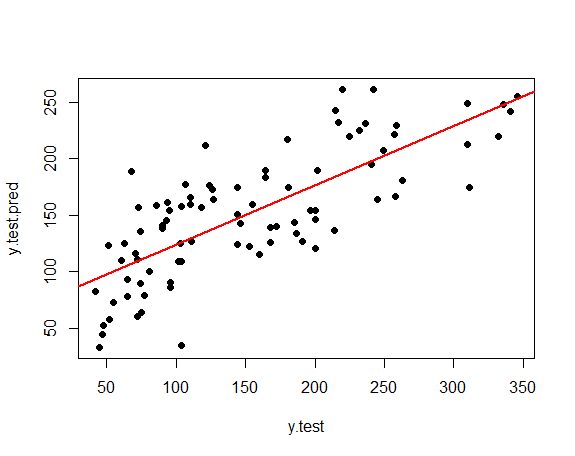
\includegraphics[width=\textwidth]{Rplot}
\caption{Biểu đồ thể hiện mối quan hệ giữa giá trị dự đoán và giá trị kiểm thử của mô hình Multiple Linear Regression} \label{fig2}
\end{figure}

\section{Kết luận}
Nhìn chung kết quả thực nghiệm trên các mô hình hồi quy vẫn còn thấp, một phần nguyên nhân là do các thuộc tính bộ dữ liệu phân bố hỗn loạn và ít có quan hệ tuyến tính với thuộc tính Y, ngoài ra còn có nhiều điểm dữ liệu ngoại lệ.

Thông qua quá trình phân tích ảnh hưởng của yếu tố lên kết quả, tương tác giữa các yếu tố và phân tích hồi quy trên bộ dữ liệu trước và sau khi tiền xử lý cho thấy rằng việc loại bỏ các điểm dữ liệu bất thường có thể làm giảm hiệu suất của mô hình. Ngoài ra, trong quá trình xây dựng mô hình, chúng tôi rút được rằng  không chỉ cần chú ý tới các yếu tố có sức ảnh hưởng lên kết quả mà cần phải quan tâm cả tới những tương tác giữa các yếu tố mặc dù những yếu tố đó khi sử dụng đơn lẻ thì không có ảnh hưởng, ví dụ điển hình trong bộ dữ liệu chính là hai thuộc tính SEX và S1. Vậy nên để mô hình đạt hiệu suất cao thì cần phải liên tục thực nghiệm trên nhiều yếu tố và tương tác khác nhau, cân nhắc xử lý các điểm dữ liệu bất thường,...

\begin{thebibliography}{5}
\bibitem{ref_url1}
Regularization: Ridge, Lasso and Elastic Net, \url{https://www.datacamp.com/community/tutorials/tutorial-ridge-lasso-elastic-net}.
\end{thebibliography}
\end{document}